\chapter{Resultados} \label{cap:resultados}

    Nesta seção serão apresentados e discutidos os resultados obtidos do desenvolvimento do trabalho tendo como base a fundamentação apresentada nos capítulos \ref{cap:id-e-controle} e \ref{cap:micromouse} e da metodologia desenvolvida no Capítuo \ref{cap:metodologia}. 
    
    Conforme será visto e detalhado nas seções a seguir, primeiro foram trabalhadas as malhas de controle internas, isto é, dos motores, realizando a devida identificação e controle, que se encontram apresentados na Seção \ref{sec:res-motores}. Posteriormente, foram trabalhadas as malhas das variáveis globais de controle cujos resultados estão apresentados na Seção \ref{sec:res-global}.

    \section{Testes realizados nos motores} \label{sec:res-motores}
        
        Inicialmente, para determinação da identificação dos motores é necessária a correta amostragem do processo dos motores. Assim, tendo como base testes experimentais e os resultados apresentados em \citeonline{tcc-marcolino}, o período de amostragem foi definido como sendo $T_s = 10ms$.

        De posse disso é produzido um sinal \gls{PRBS} em torno de um valor central de referência $R$ usando um valor de margem $\varDelta x = 0.1R$. Este sinal é empregado em identificação de sistemas por apresentar características semelhantes às de um ruído aleatório sendo, entretanto, determinístico e reprodutível. Dessa forma, é possível excitar o sistema em uma ampla faixa de frequências, permitindo evidenciar sua dinâmica.
        
        % O sinal é construído usando um registrador de deslocamento \gls{LFSR} dentro do microcontrolador juntamente da operação lógica \textit{XOR}. A regra que define a saída do \gls{PRBS} é apresentado na Equação \ref{eq:deslocamento-bit}. A saída possui dois níveis lógicos de forma que se $b(k) = 1$ a resposta produz um sinal $R + \varDelta x$, e se $b(k) = 0$ é produzido um sinal $R - \varDelta x$, o que pode ser definido pela Equação \ref{eq:saida-prbs}.

        Neste trabalho, o sinal é gerado por meio de um registrador de deslocamento com realimentação linear -- \gls{LFSR} -- implementado no microcontrolador. A sequência binária é produzida a partir da operação lógica \textit{XOR} entre posições específicas do registrador. Embora a sequência gerada seja periódica, seu período é suficientemente elevado para que, durante os experimentos, apresente comportamento semelhante ao de um sinal aleatório.

        A saída do \gls{PRBS} possui dois níveis lógicos. Quando $b(k)=1$, o sinal de entrada assume o valor $R+\varDelta x$, enquanto para $b(k)=0$ a entrada passa a assumir o valor $R-\varDelta x$. A regra de geração da sequência binária é apresentada na Equação \ref{eq:deslocamento-bit}, enquanto a definição do sinal aplicado ao sistema é dada pela Equação~\ref{eq:saida-prbs}.

        \begin{equation}
            \label{eq:deslocamento-bit}
            b(k) = s_{15}(k)\oplus s_{14}(k)
        \end{equation}

        \begin{equation}
            \label{eq:saida-prbs}
            u(k) = 
            \begin{cases}
                R + \varDelta x, & b(k) = 1 \\
                R - \varDelta x, & b(k) = 0
            \end{cases}
        \end{equation}
        
        \subsection{Identificação dos motores} \label{sec:res-id-motores}

            Assim, um sinal \gls{PRBS} com $R = 50\%$ é aplicado a cada um dos motores e suas resposta são coletadas e apresentadas nas Figuras \ref{fig:saida-prbs-motor-direito} e \ref{fig:saida-prbs-motor-esquerdo}. Nestas figuras estão apresentados o sinal de entrada, em vermelho, aplicado aos motores e o sinal de resposta de cada um deles, na cor preta.  
            
            \begin{figure}[htb]
                \centering
                \Caption{\label{fig:saida-prbs-motor-direito} Resposta do motor direito}	
                    \UFCfig{}{
                        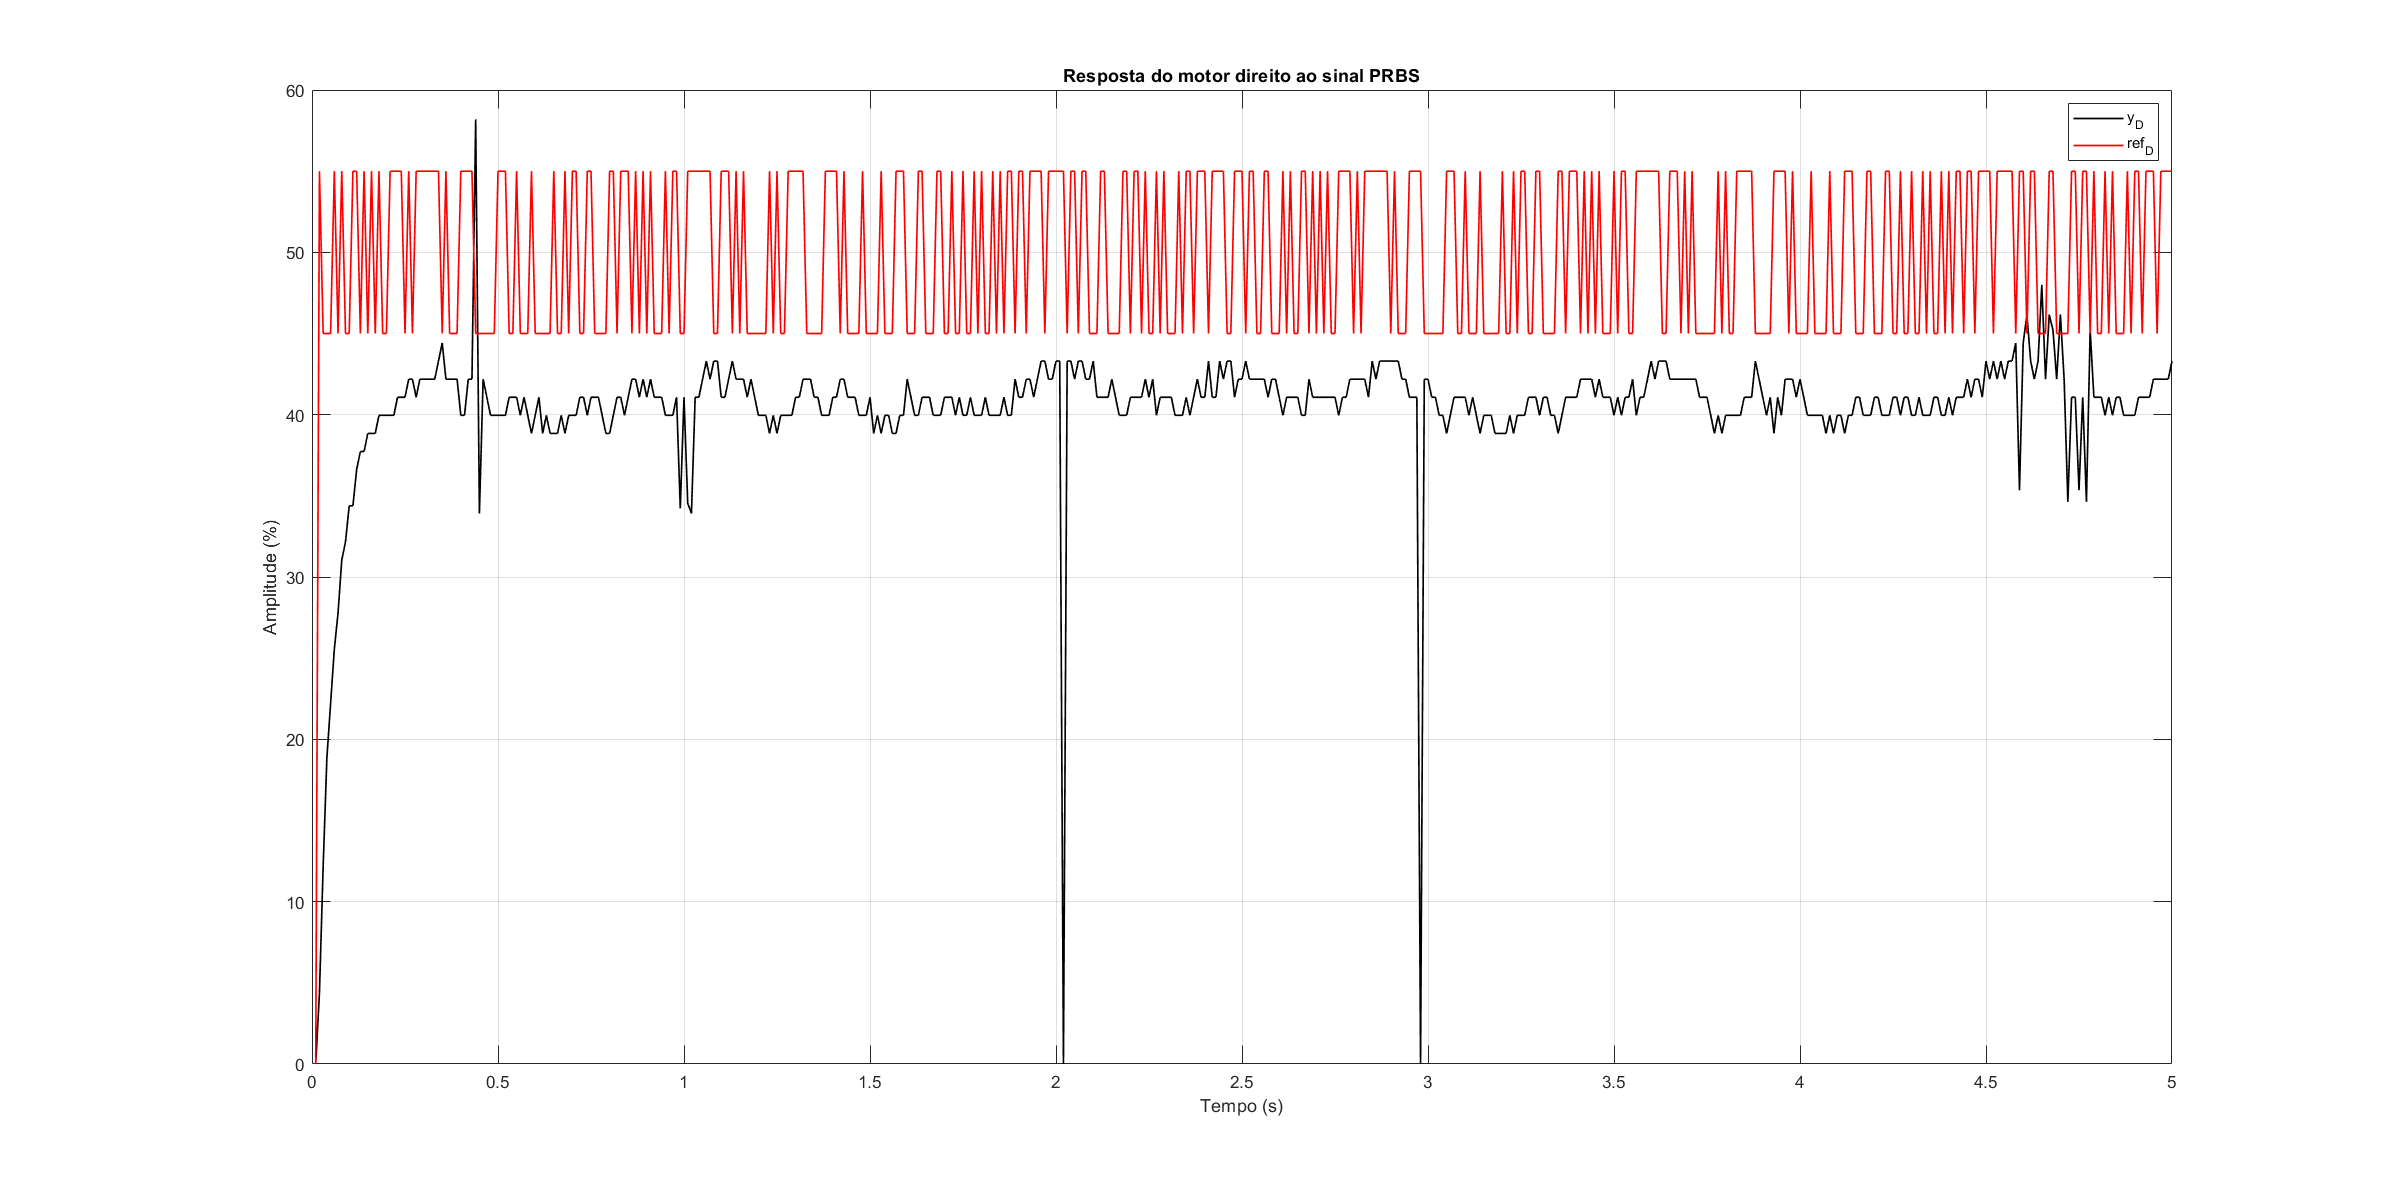
\includegraphics[width=16cm]{figuras/resultados/fig-motores/resp_mot_dir_prbs.png}
                    }{
                        \Fonte{O autor}
                    }	
            \end{figure}

            \begin{figure}[htb]
                \centering
                \Caption{\label{fig:saida-prbs-motor-esquerdo} Resposta do motor esquerdo}	
                    \UFCfig{}{
                        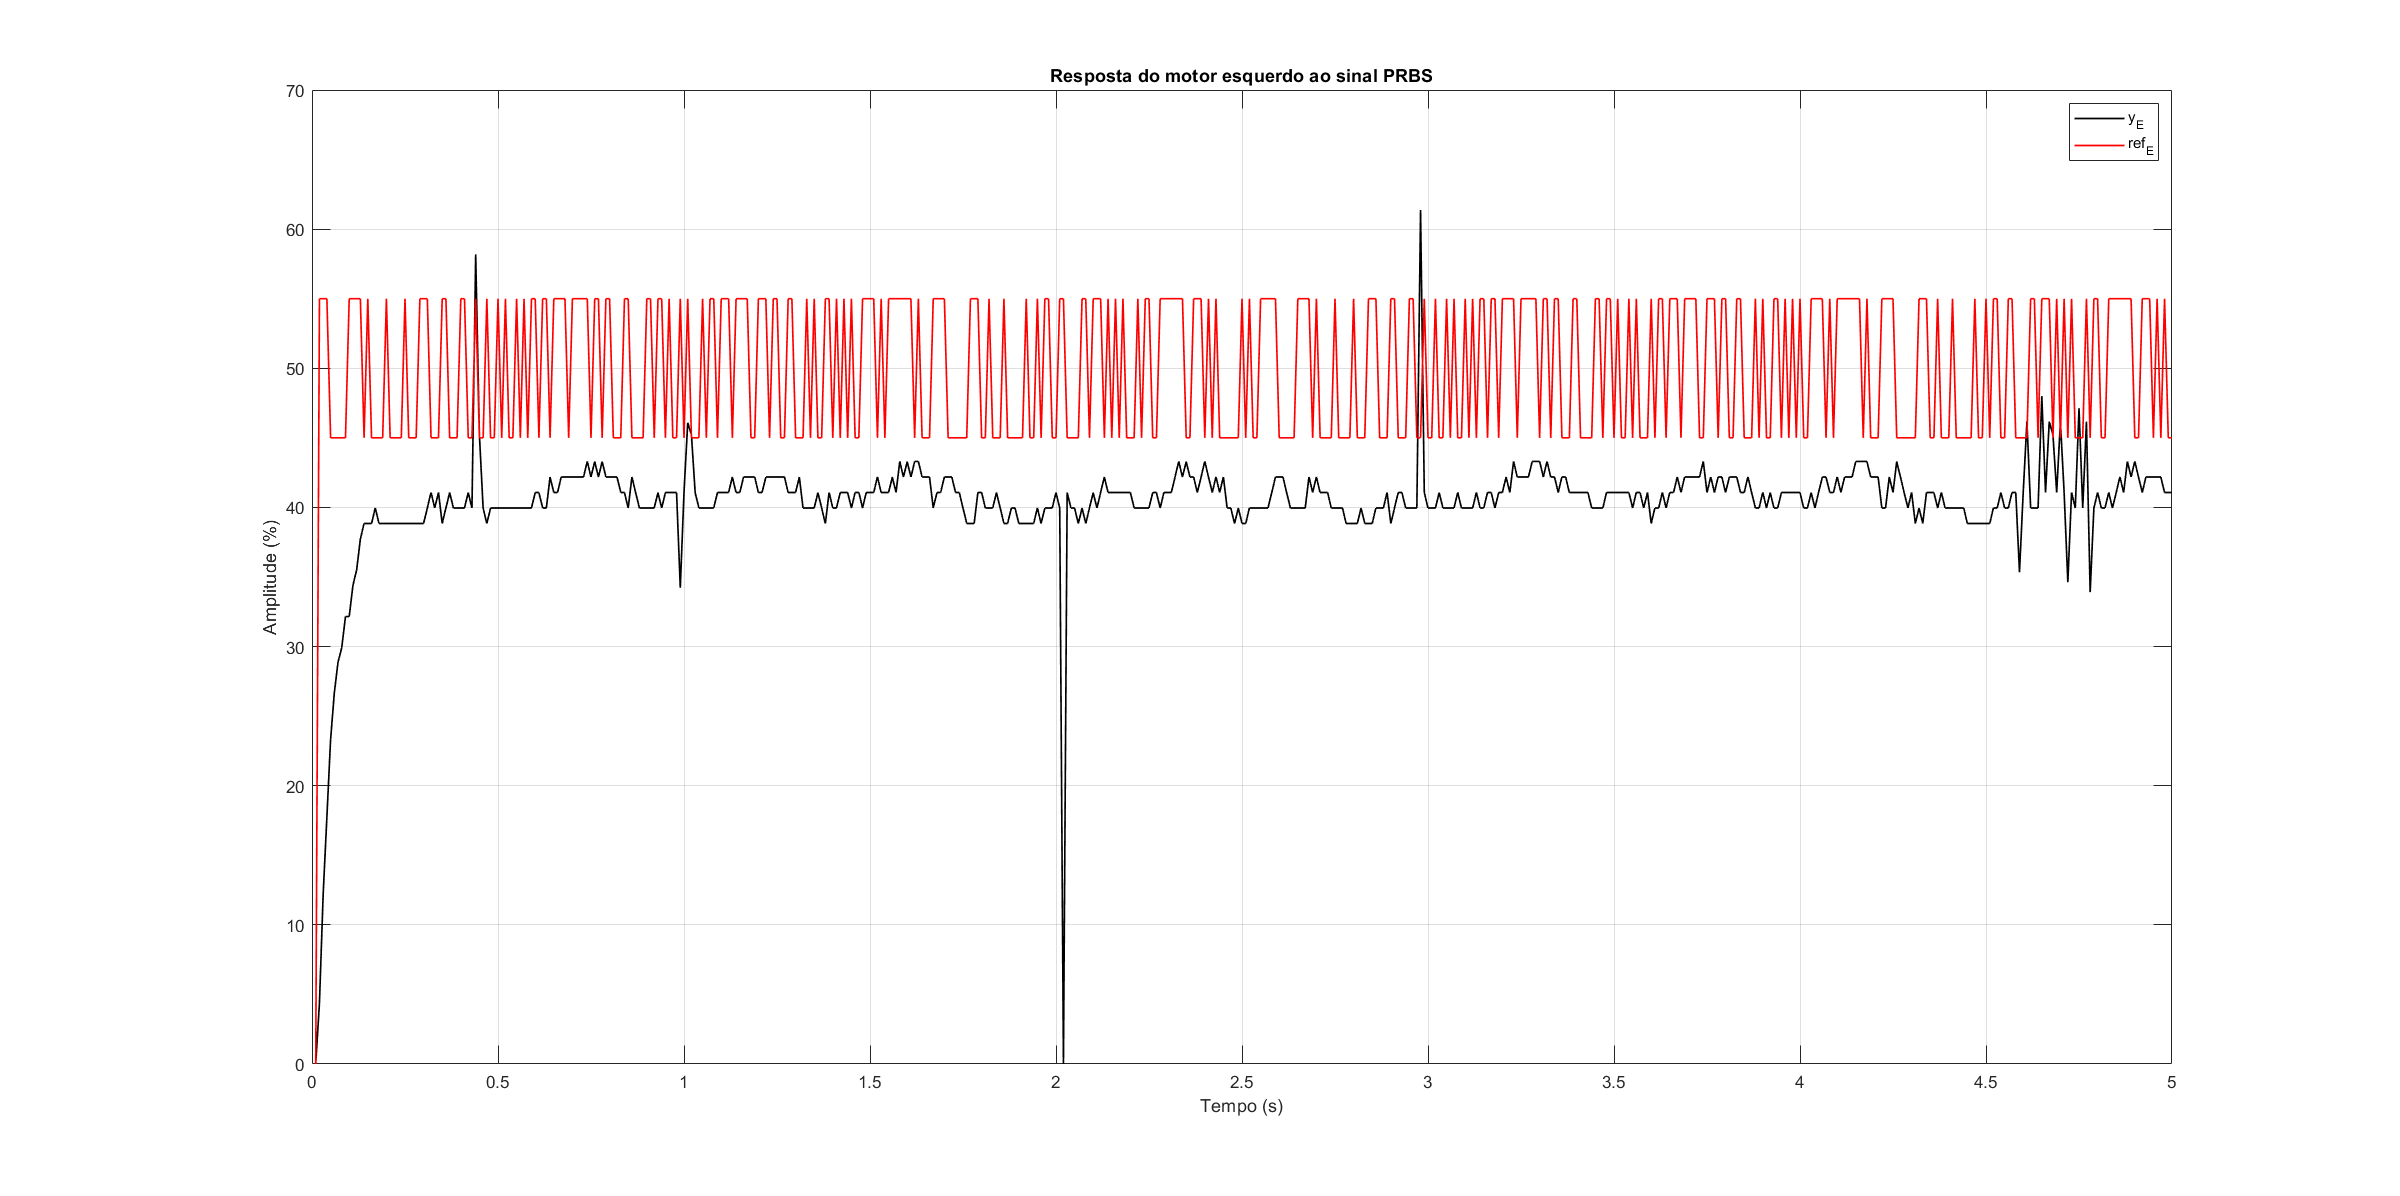
\includegraphics[width=16cm]{figuras/resultados/fig-motores/resp_mot_esq_prbs.png}
                    }{
                        \Fonte{O autor}
                    }	
            \end{figure}
            
            Com os dados coletados é possível então a aplicação do método \gls{MQNR} para identificação e construção dos modelos metamáticos de cada um dos motores conforme a Equação \ref{eq:ft-ordem-2-z-com-atraso}. Os resultados usados para validas as respectivas identificações são apresentados nas Figuras \ref{fig:identificacao-motor-direito} e \ref{fig:identificacao-motor-esquerdo}. Em cada uma das figuras estão contidos dois \textit{plots}, onde o superior contém, em preto, o sinal de resposta do motor, também apresentado nas figuras anteriores, e, em vermelho, o sinal obtido da aplicação dos modelos obtidos. Já no segundo \textit{plot}, em azul, está apresentado o sinal de erro de identificação, correspondendo à diferença entre a saída real e a saída modelada.

            \begin{figure}[ht]
                \centering
                \Caption{\label{fig:identificacao-motor-direito} Identificação do motor direito}	
                    \UFCfig{}{
                        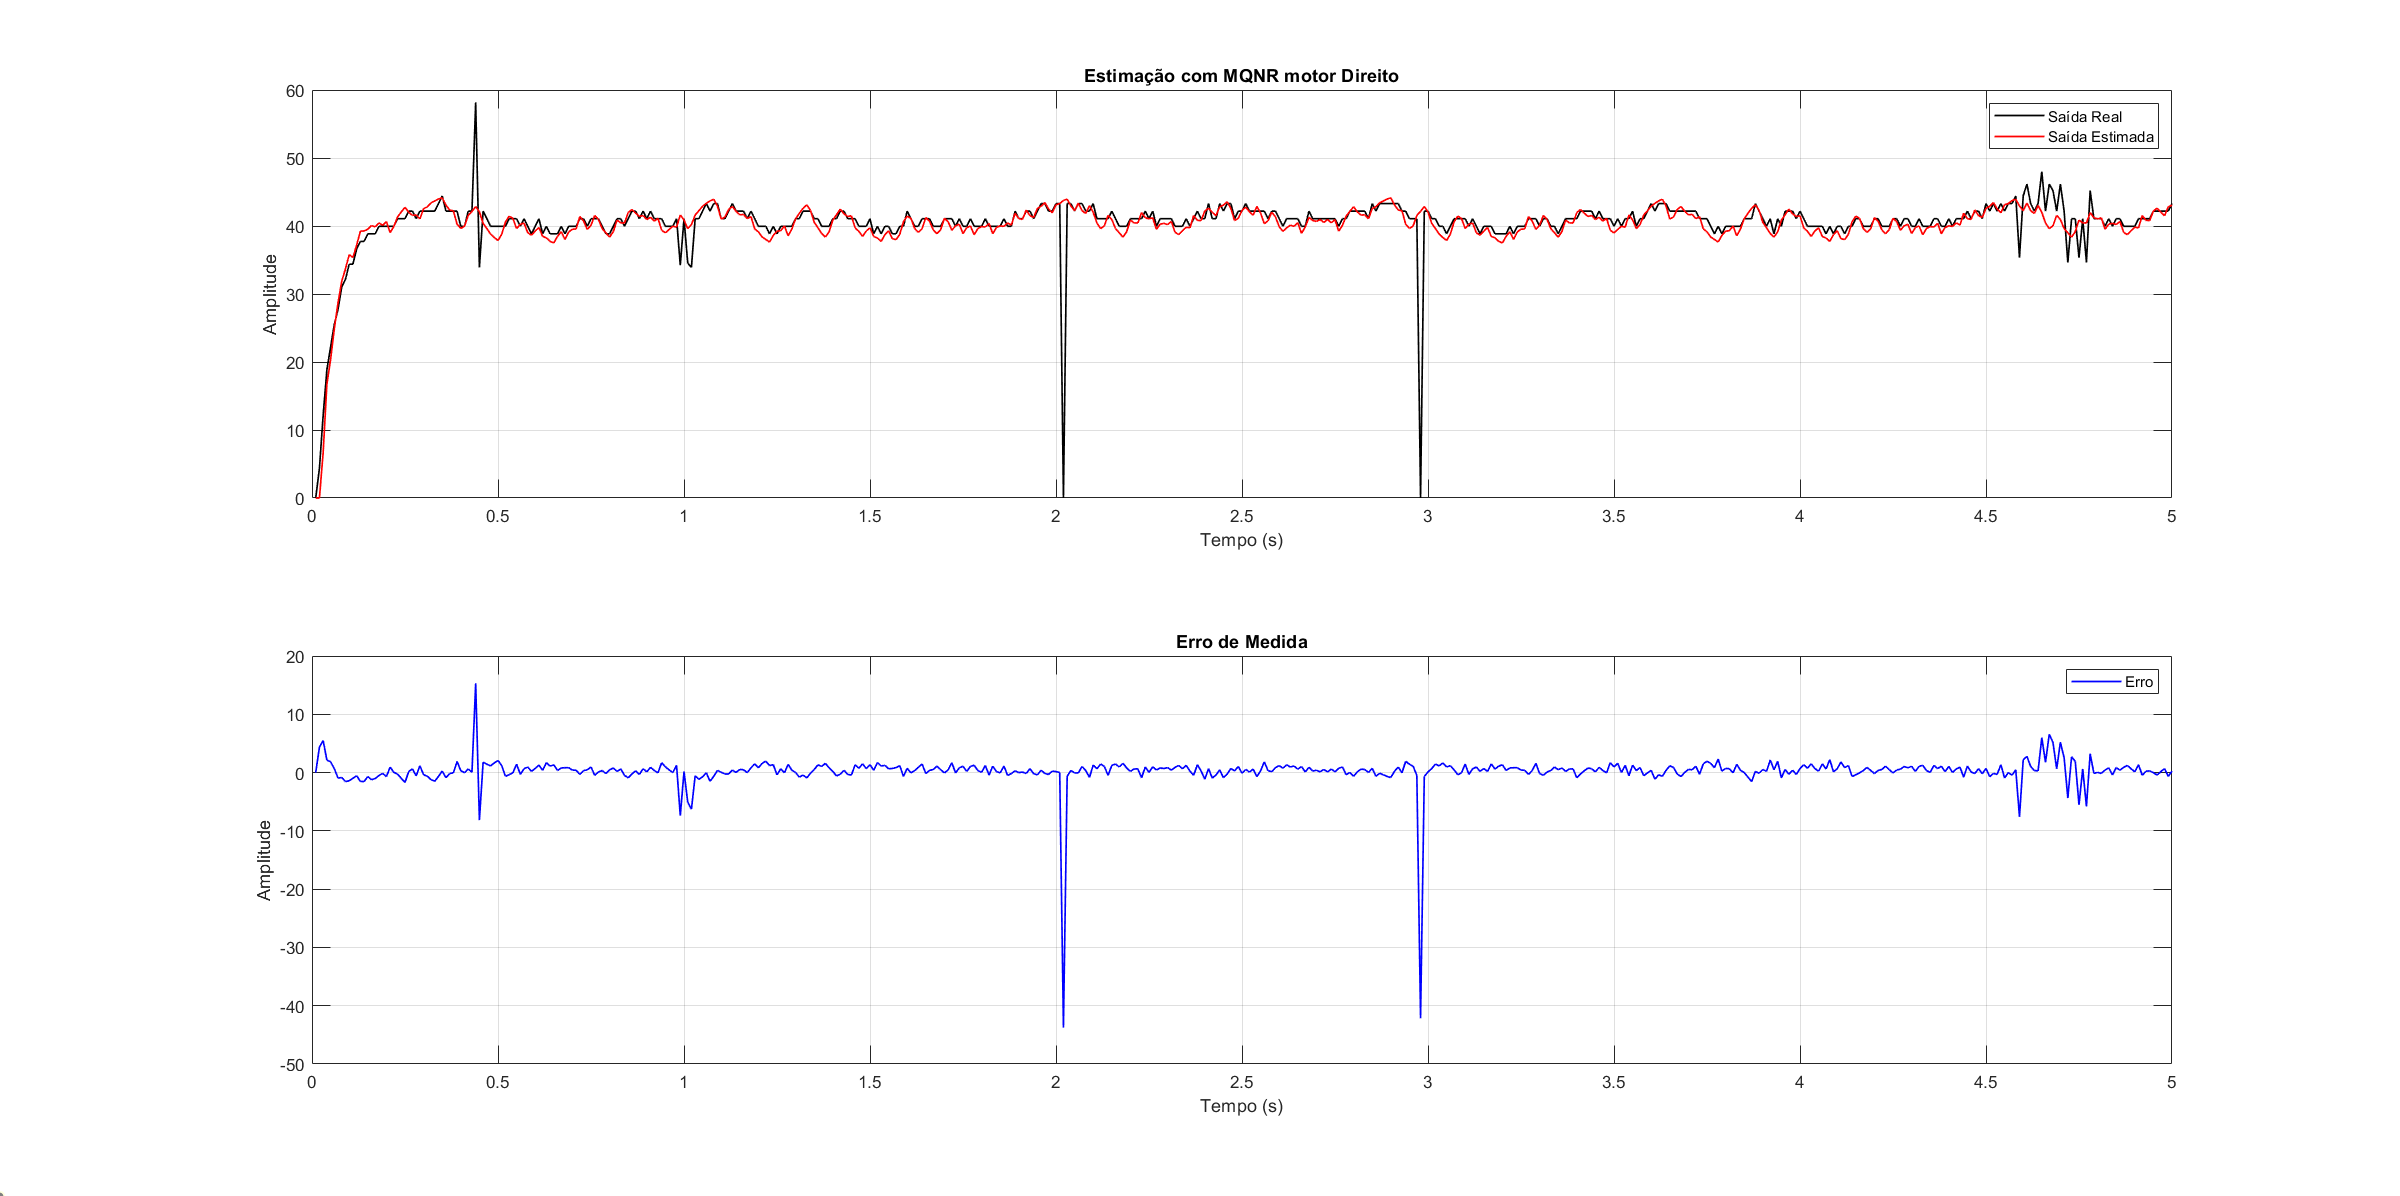
\includegraphics[width=16cm]{figuras/resultados/fig-motores/identifica_motor_direito.png}
                    }{
                        \Fonte{O autor}
                    }	
            \end{figure}

            \begin{figure}[ht]
                \centering
                \Caption{\label{fig:identificacao-motor-esquerdo} Identificação do motor esquerdo}	
                    \UFCfig{}{
                        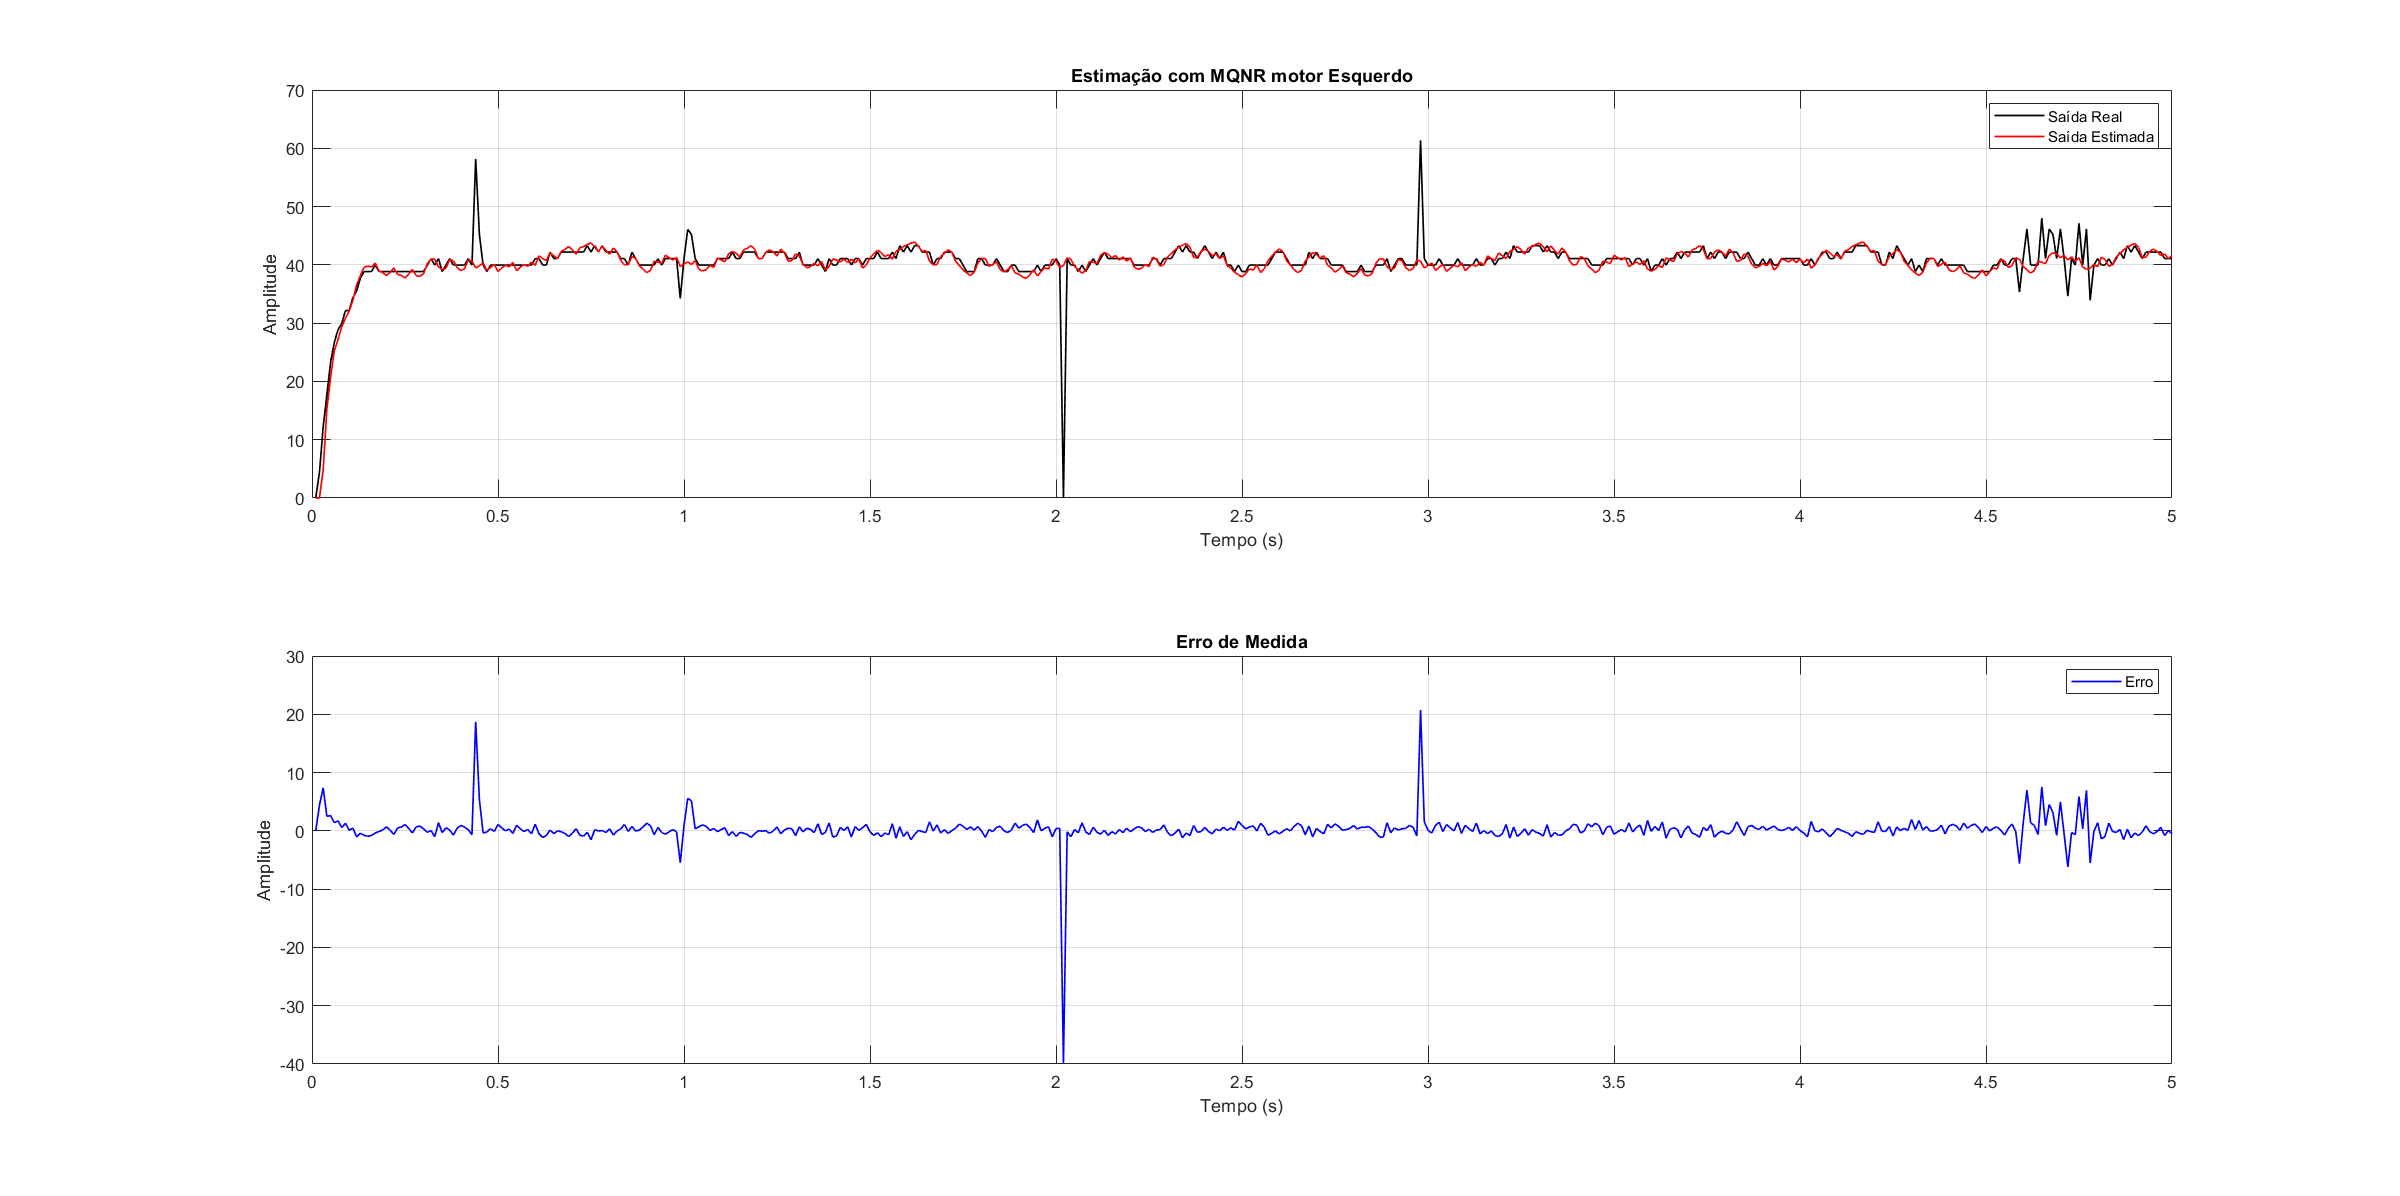
\includegraphics[width=16cm]{figuras/resultados/fig-motores/identifica_motor_esquerdo.png}
                    }{
                        \Fonte{O autor}
                    }	
            \end{figure}

            É possível observar que, para ambos os casos, o método aplicado obtém uma resposta que pode ser considerada satisfatória, haja vista que o gráfico do erro de identificação encontra-se próximo de zero, com exceção dos pontos de ruído de medição os quais não são representados pelo modelo, fazendo com que, nesses pontos, o erro seja maior. Os coeficientes obtidos da identificação de cada um dos motores são apresentados a seguir na Tabela \ref{tab:identificacao-motores}.

            \begin{table}[!htbp]	
				\centering
				\Caption{\label{tab:identificacao-motores} Coeficientes dos modelos dos motores}
				\UFCtab{}{
					\begin{tabular}{ccc}
						\toprule
						Coeficiente/Motor & \( Direito \) & \( Esquerdo \) \\
						\midrule
						\( a_1 \) & \( -0.3101 \) & \( -0.2496 \) \\
						\( a_2 \)    & \( -0.3252 \) & \( -0.3680 \) \\
						\( b_1 \)   & \( 0.1326 \) & \( 0.1281 \) \\
                        \( b_2 \)   & \( 0.1651 \) & \( 0.1821 \) \\
						\bottomrule
					\end{tabular}
				}{
					\Fonte{O autor}
				}
			\end{table}

        \subsection{Controle aplicado nos motores} \label{sec:res-controle-motores}

            Com os modelos em mãos, é possível prosseguir para a etapa de projeto dos controladores a partir do método do Relé. Os resultados da aplicação de um relé em cada um dos modelos dos motores são apresentados nas Figuras \ref{fig:rele-modelo-direito} e \ref{fig:rele-modelo-esquerdo} e os parâmetros utilizados são apresentados na Tabela \ref{tab:parametros-rele-motores}. Em cada uma das Figuras \ref{fig:rele-modelo-direito} e \ref{fig:rele-modelo-esquerdo} é possível observar três sinais: o sinal de referência, em verde, o sinal de entrada do Relé, em preto, e o sinal da resposta do sistema modelado ao Relé, em vermelho.
            
            \begin{figure}[ht]
                \centering
                \Caption{\label{fig:rele-modelo-direito} Relé no modelo do motor direito}	
                    \UFCfig{}{
                        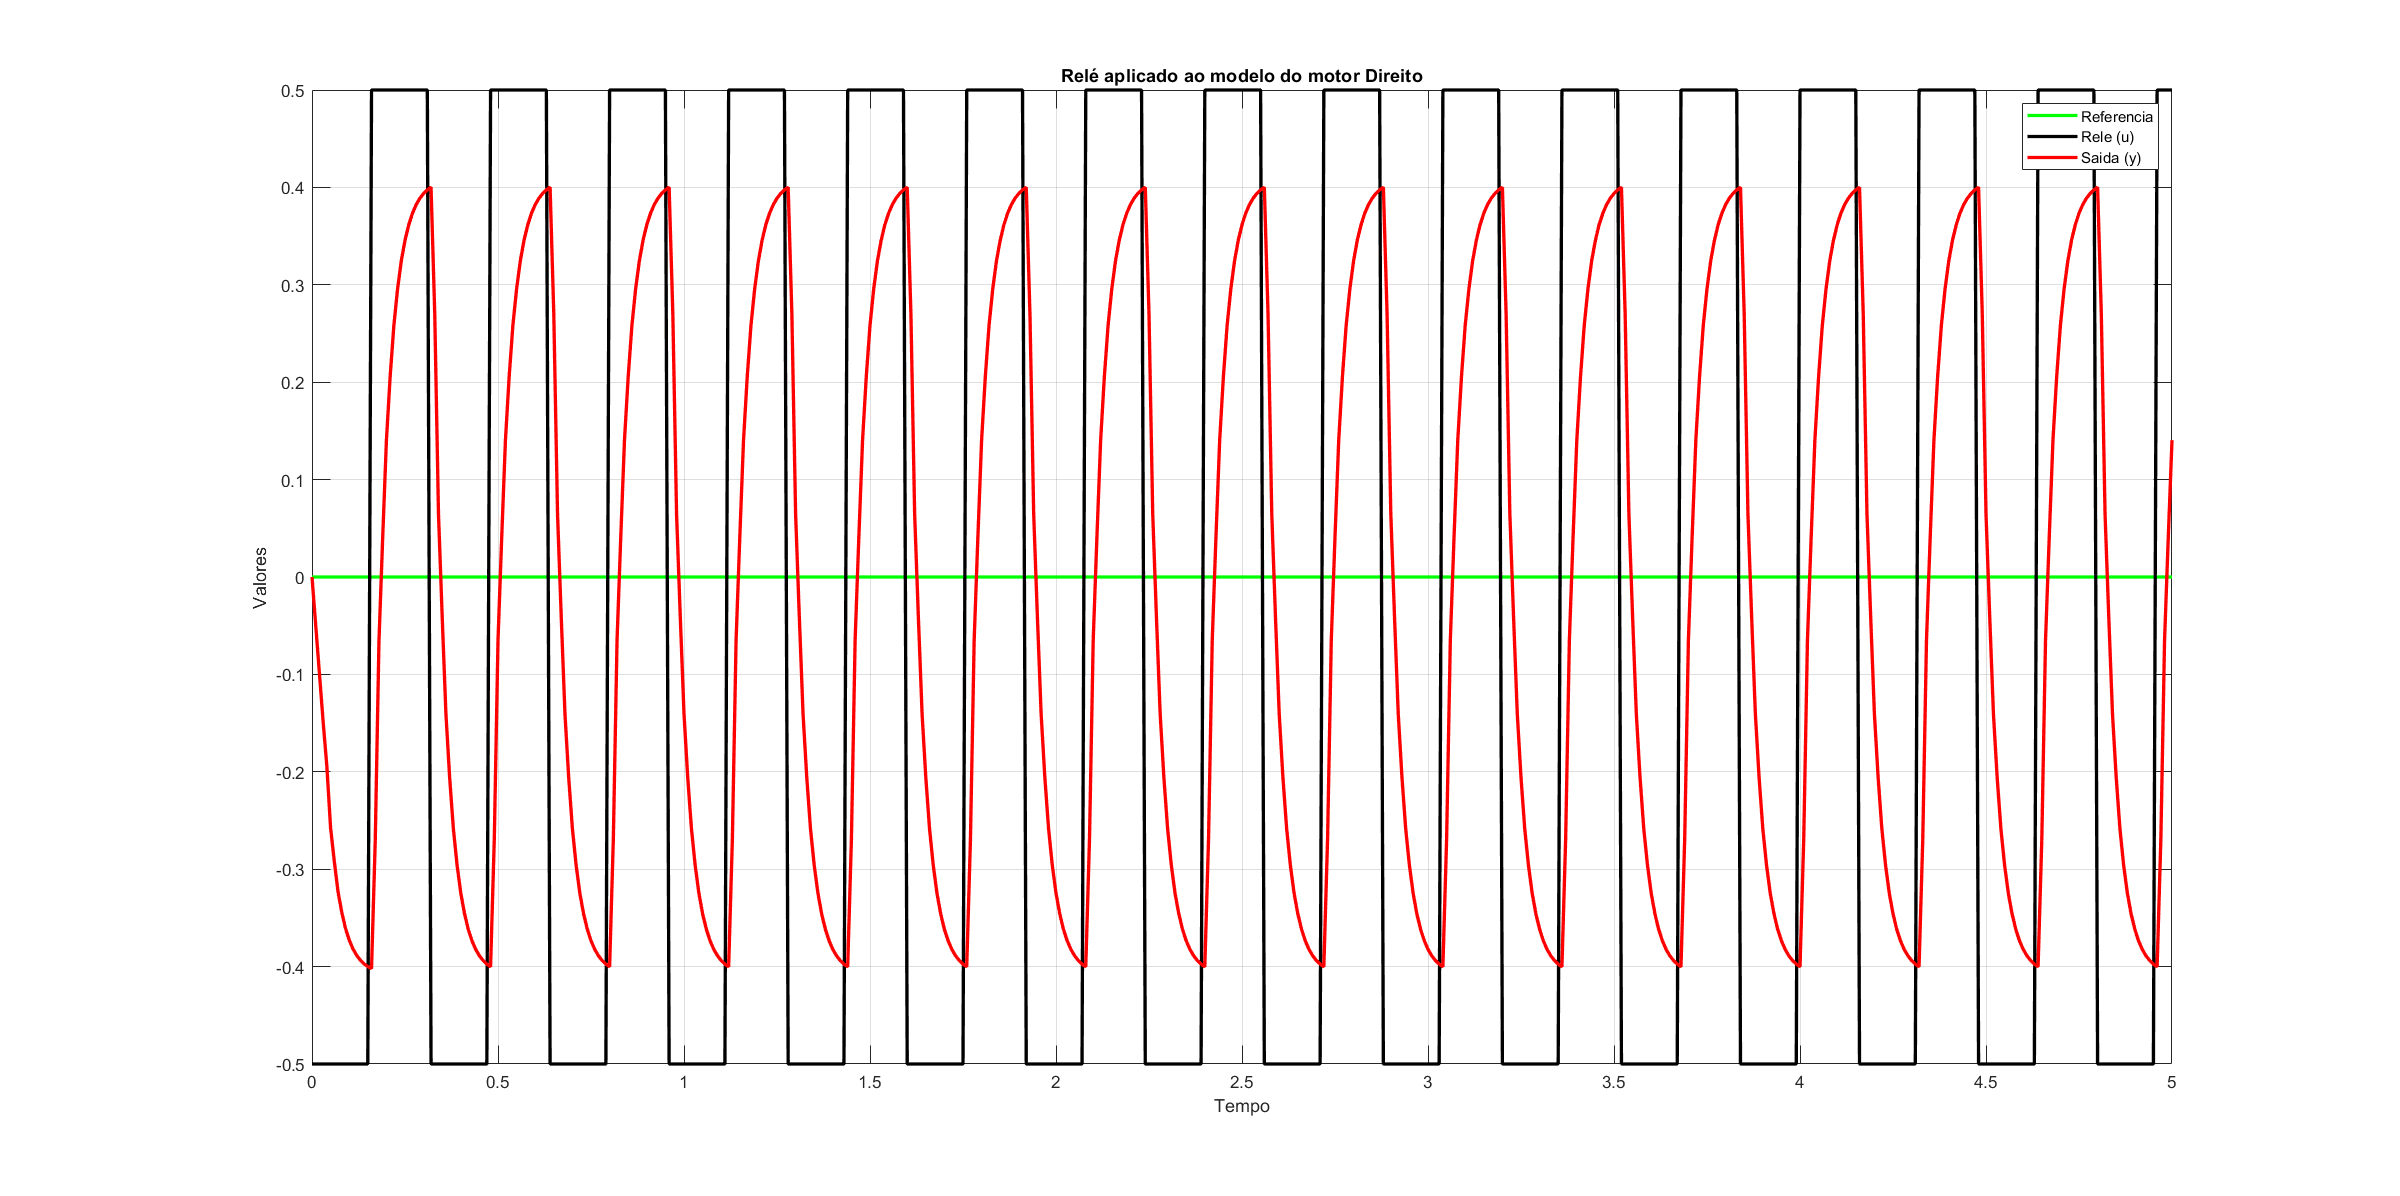
\includegraphics[width=16cm]{figuras/resultados/fig-motores/rele_motor_direito.png}
                    }{
                        \Fonte{O autor}
                    }	
            \end{figure}

            \begin{figure}[ht]
                \centering
                \Caption{\label{fig:rele-modelo-esquerdo} Relé no modelo do motor esquerdo}	
                    \UFCfig{}{
                        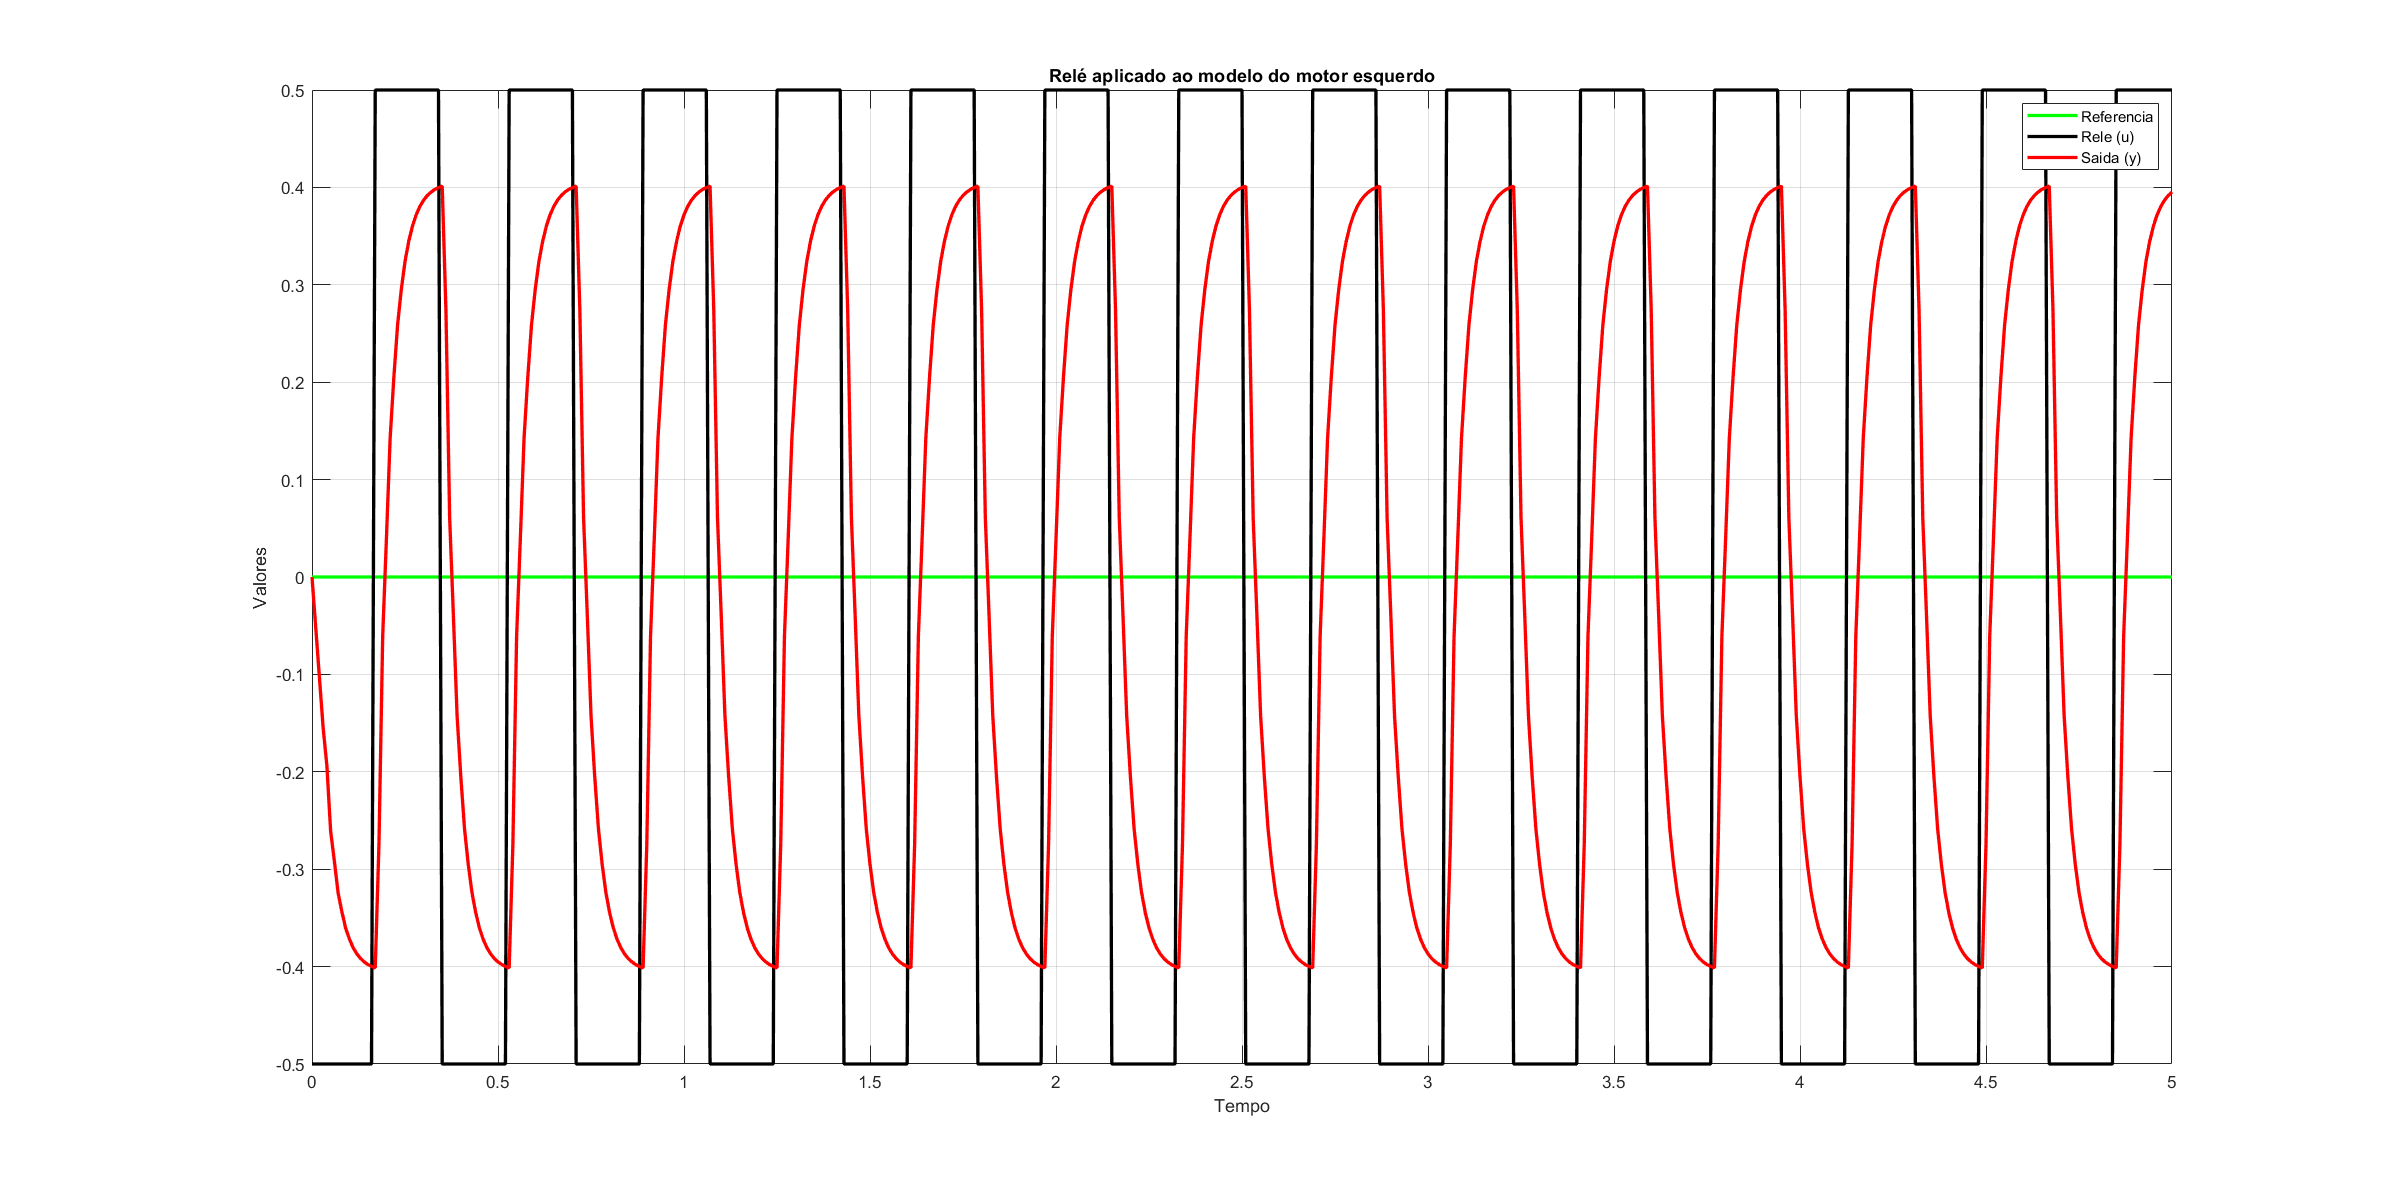
\includegraphics[width=16cm]{figuras/resultados/fig-motores/rele_motor_esquerdo.png}
                    }{
                        \Fonte{O autor}
                    }	
            \end{figure}

            \begin{table}[!htbp]	
				\centering
				\Caption{\label{tab:parametros-rele-motores} Parâmetros do Relé para os motores}
				\UFCtab{}{
					\begin{tabular}{ccc}
						\toprule
						Parâmetro/Motor & \( Direito \) & \( Esquerdo \) \\
						\midrule
						\( K_{u} \) & \( 1.5910 \) & \( 1.5864 \) \\
						\( T_{u} \)    & \( 0.3200 \) & \( 0.3600 \) \\
						\( a \)   & \( 0.4001 \) & \( 0.4013 \) \\
                        \( d \)   & \( 0.5000 \) & \( 0.5000 \) \\
                        \( \epsilon \)   & \( 0.4000 \) & \( 0.4000 \) \\
                        \( \omega_{u} \)   & \( 19.6350 \) & \( 17.4553 \) \\
						\bottomrule
					\end{tabular}
				}{
					\Fonte{O autor}
				}
			\end{table}

            Observa-se que os modelos possuem dinâmicas parecidas, porém não podem ser consideradas iguais de forma que os resultados da aplicação do relé resultam em parâmetros ligeiramente diferentes, o que resultará também en controladores com diferentes ganhos.

            Por fim, são projetados os controladores, cujos parâmetros $g_0$, $g_1$ e $g_2$ são obtidos para cada um dos motores e aplicados no robô e mostrados conforme a Tabela \ref{tab:parametros-controladores-motores}.

            \begin{table}[!htbp]	
				\centering
				\Caption{\label{tab:parametros-controladores-motores} Parâmetros do controlador para os motores}
				\UFCtab{}{
					\begin{tabular}{ccc}
						\toprule
						Parâmetro/Motor & \( Direito \) & \( Esquerdo \) \\
						\midrule
						\( g_0 \) & \( 2.2859 \) & \( 3.4699 \) \\
						\( g_1 \)    & \( -3.4750 \) & \( -5.4859 \) \\
						\( g_2 \)   & \( 1.3341 \) & \( 2.1822 \) \\
						\bottomrule
					\end{tabular}
				}{
					\Fonte{O autor}
				}
			\end{table}

            Os testes de controle foram conduzidos aplicando inicialmente um patamar de referência e depois aplicando três patamares, conforme apresentado nas Figuras \ref{fig:controle-motor-direito-1-patamar} a \ref{fig:controle-motor-esquerdo-3-patamares}. Suas métricas são então apresentadas nas Tabelas \ref{tab:metricas-controle-1-patamar} e \ref{tab:metricas-controle-3-patamares}.

            As Figuras \ref{fig:controle-motor-direito-1-patamar} a \ref{fig:controle-motor-esquerdo-3-patamares} também contém dois \textit{plots}. No primeiro está contido o sinal de referência, em azul, a resposta dos motores, em preto, e o erro do sistema, em rosa. No segundo \textit{plot} está contida a o sinal de controle produzido por cada um dos controladores \gls{PID} e que corresponde à entrada do motor.

            \begin{figure}[ht]
                \centering
                \Caption{\label{fig:controle-motor-direito-1-patamar} PID no motor direito para 1 patamar}	
                    \UFCfig{}{
                        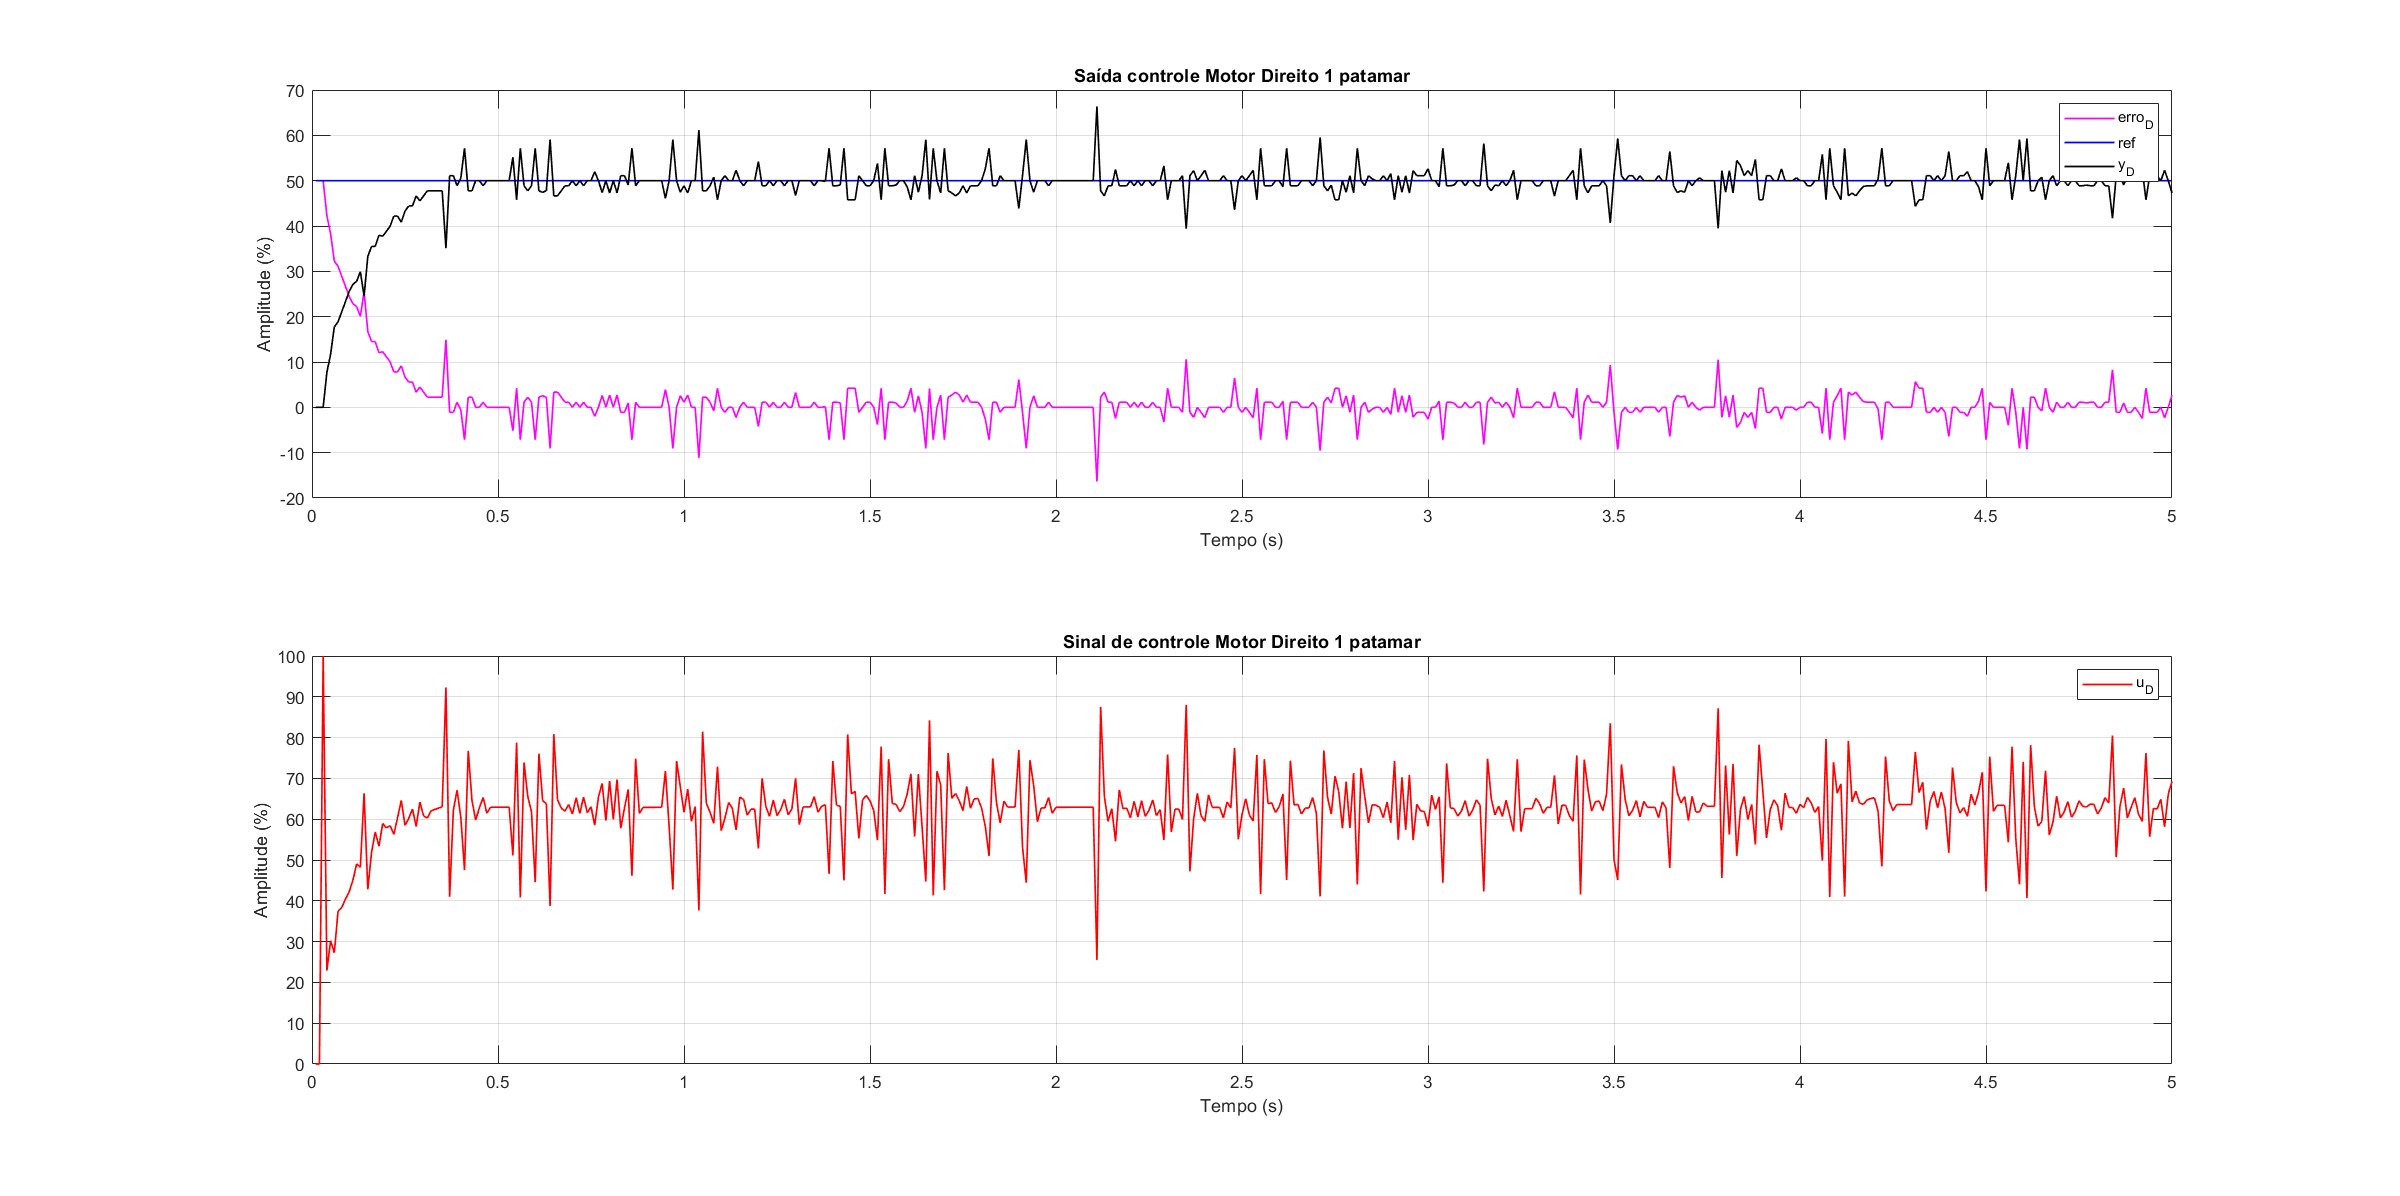
\includegraphics[width=16cm]{figuras/resultados/fig-motores/PID_direito_1_patamar_sem_ressintonia.png}
                    }{
                        \Fonte{O autor}
                    }	
            \end{figure}

            \begin{figure}[ht]
                \centering
                \Caption{\label{fig:controle-motor-esquerdo-1-patamar} PID no motor esquerdo para 1 patamar}	
                    \UFCfig{}{
                        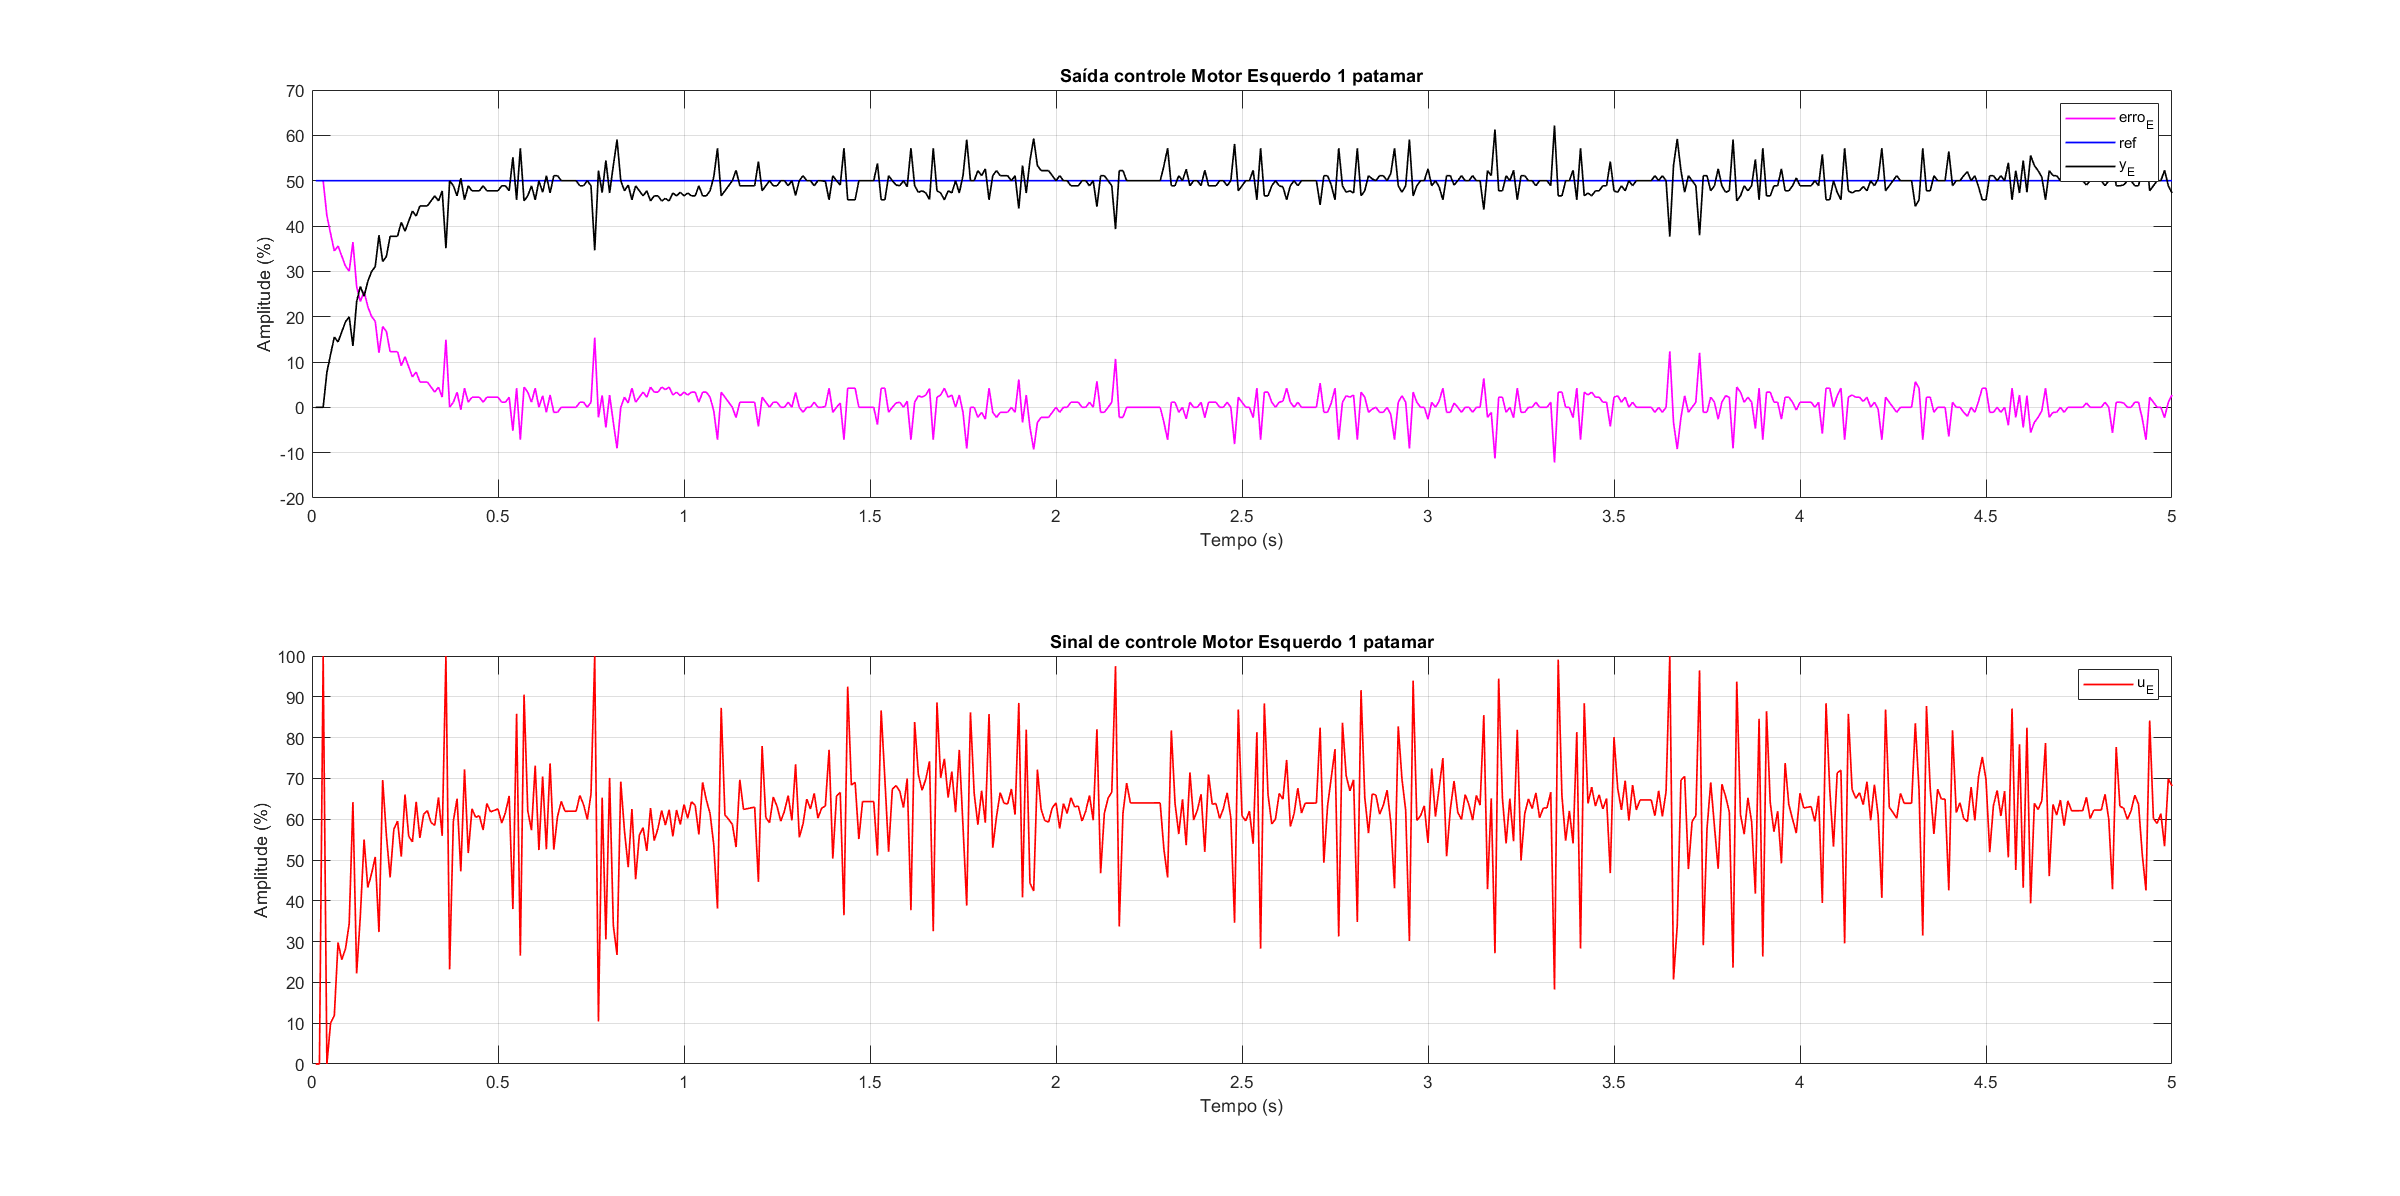
\includegraphics[width=16cm]{figuras/resultados/fig-motores/PID_esquerdo_1_patamar_sem_ressintonia.png}
                    }{
                        \Fonte{O autor}
                    }	
            \end{figure}

            \begin{figure}[ht]
                \centering
                \Caption{\label{fig:controle-motor-direito-3-patamares} PID no motor direito para 3 patamares}	
                    \UFCfig{}{
                        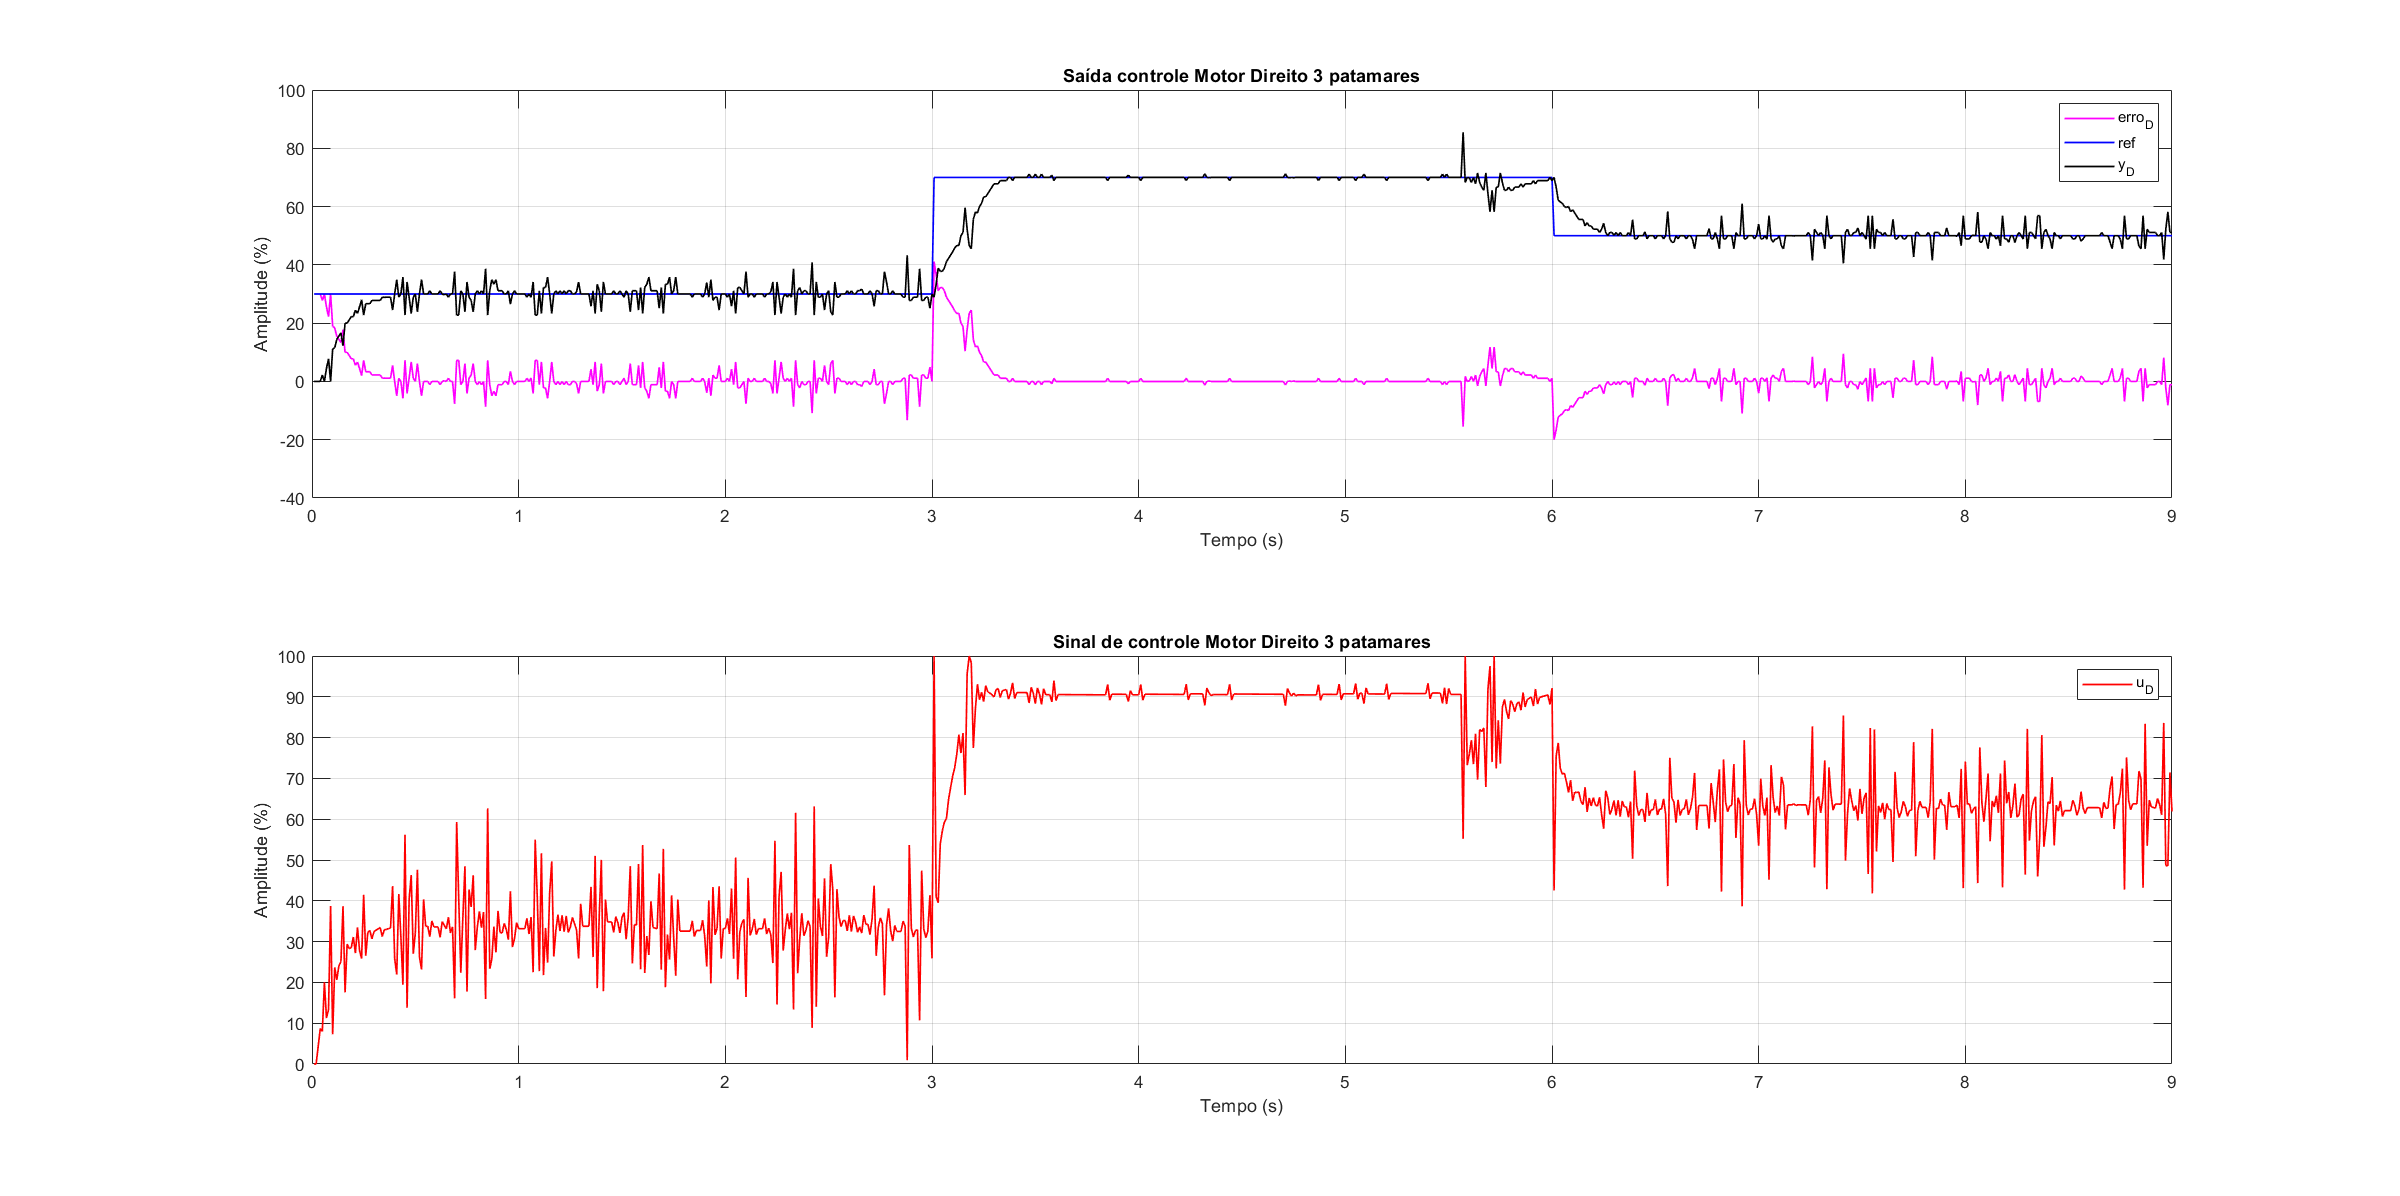
\includegraphics[width=16cm]{figuras/resultados/fig-motores/PID_direito_3_patamar_sem_ressintonia.png}
                    }{
                        \Fonte{O autor}
                    }	
            \end{figure}

            \begin{figure}[ht]
                \centering
                \Caption{\label{fig:controle-motor-esquerdo-3-patamares} PID no motor esquerdo para 3 patamares}	
                    \UFCfig{}{
                        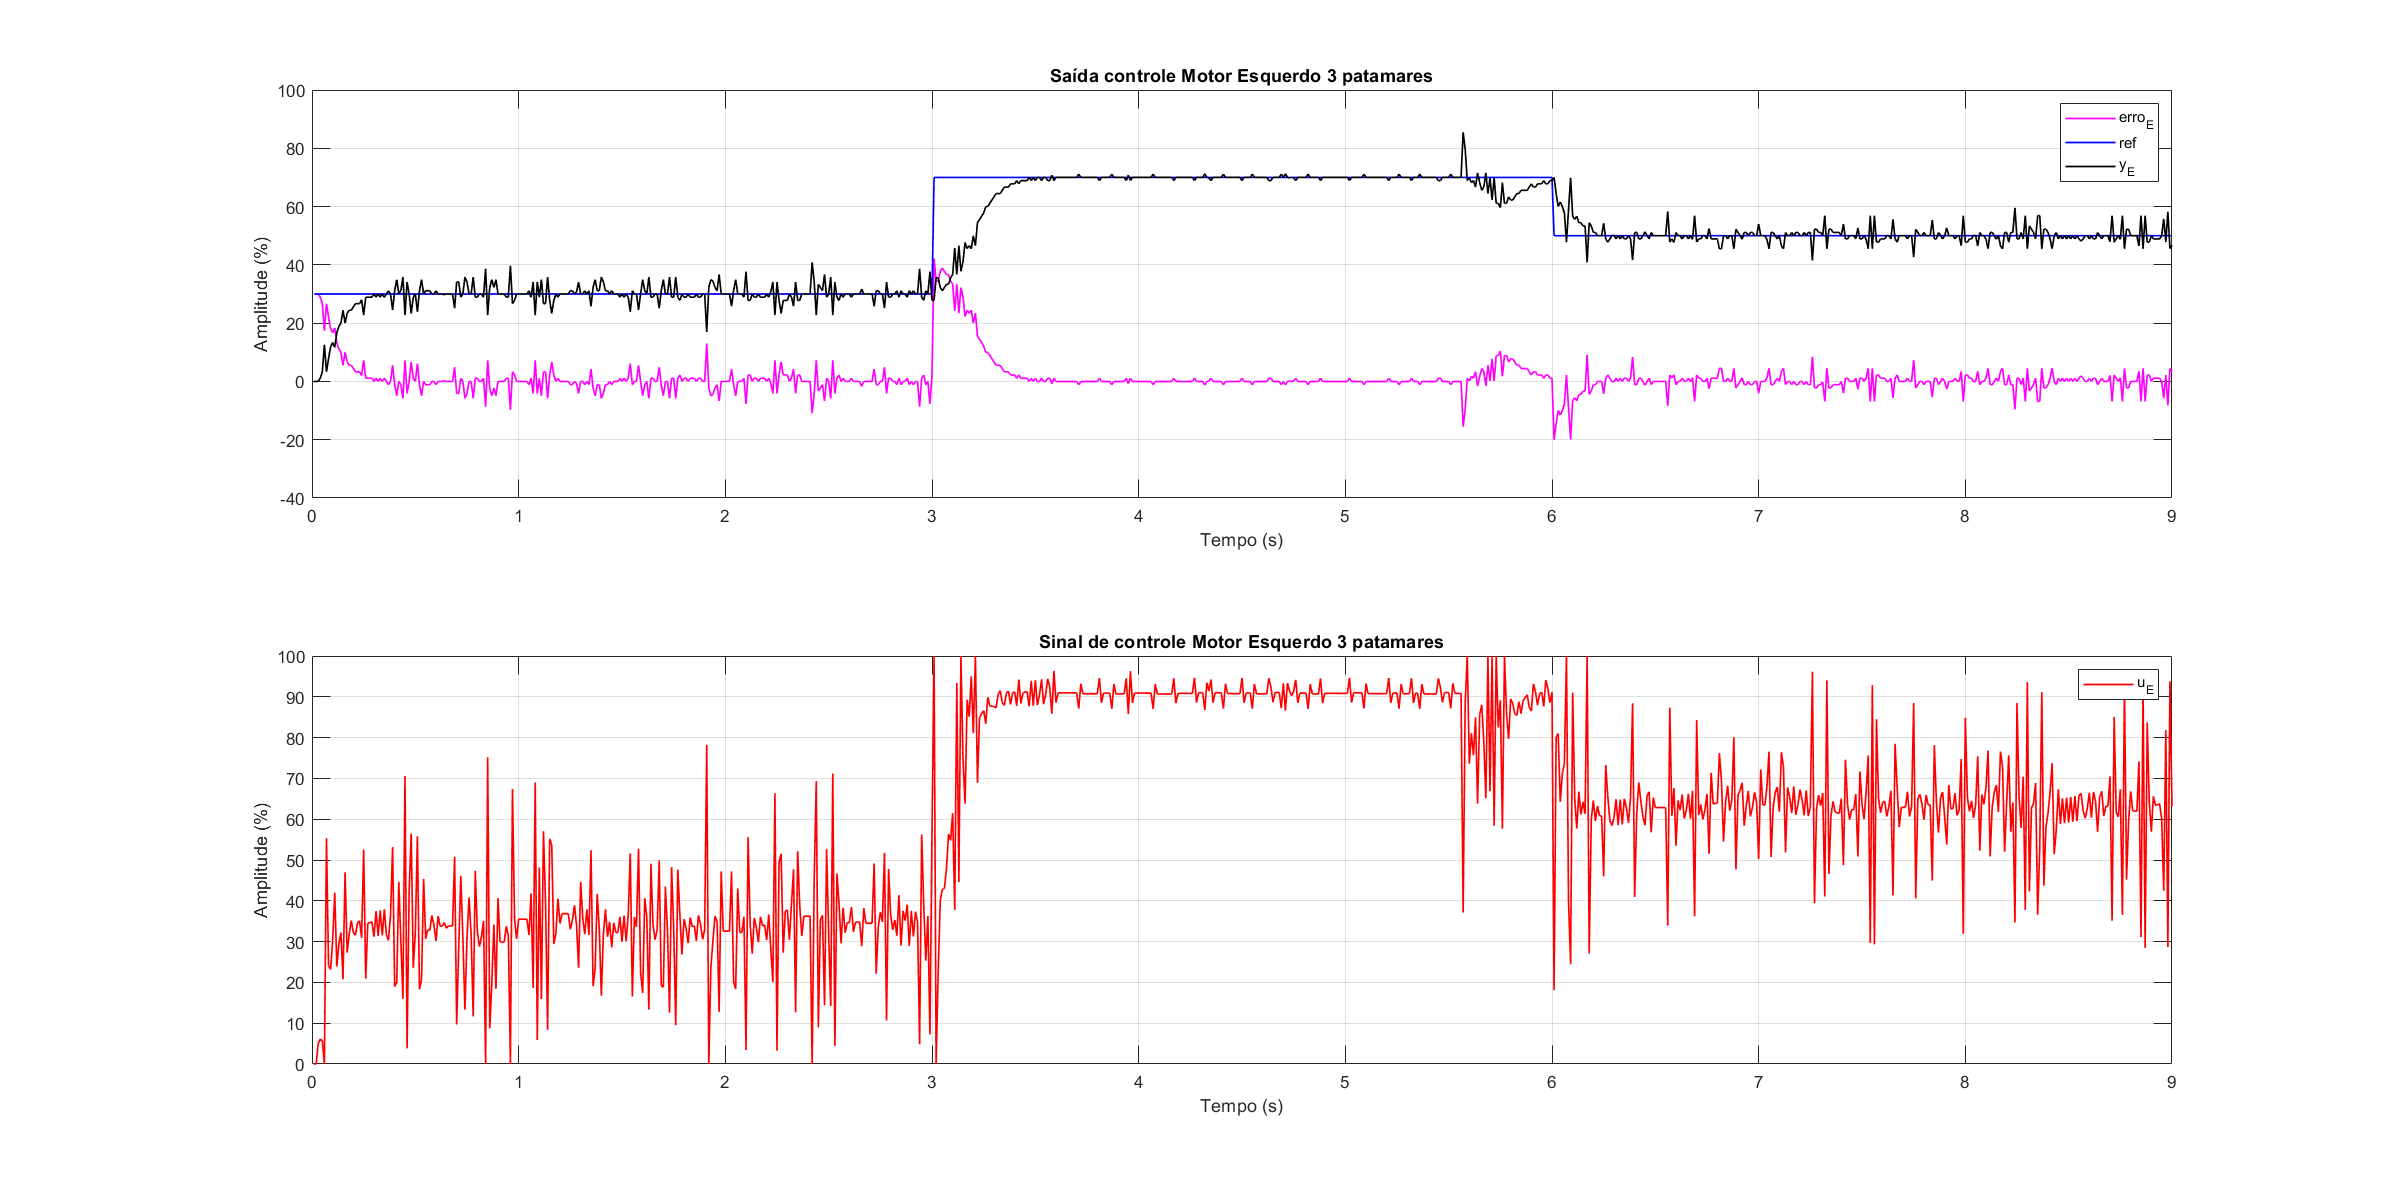
\includegraphics[width=16cm]{figuras/resultados/fig-motores/PID_esquerdo_3_patamar_sem_ressintonia.png}
                    }{
                        \Fonte{O autor}
                    }	
            \end{figure}

            \begin{table}[!htbp]	
				\centering
				\Caption{\label{tab:metricas-controle-1-patamar} Resultados de controle para 1 patamar}
				\UFCtab{}{
					\begin{tabular}{ccc}
						\toprule
						    Métrica/Motor & Direito & Esquerdo \\
						\midrule
                            Sobressinal (\%) & \( 2.2064 \) & \( 24.3352 \) \\
                            IAE & \( 1436.6 \) & \( 1700.1 \) \\
                            Variância da saída & \( 43.9402 \) & \( 50.9943 \) \\
                            Variância da do controle & \( 94.5763 \) & \( 214.4647 \) \\
                            Tempo de assentamento (s) & \( 0.3600 \) & \( 0.3900 \) \\
						\bottomrule
					\end{tabular}
				}{
					\Fonte{O autor}
				}
			\end{table}

            \begin{table}[!htbp]	
				\centering
				\Caption{\label{tab:metricas-controle-3-patamares} Resultados de controle para 3 patamares}
				\UFCtab{}{
					\begin{tabular}{ccc}
						\toprule
						    Métrica/Motor & Direito & Esquerdo \\
						\midrule
                            Sobressinal do primeiro patamar (\%) & \( 3.7327 \) & \( 0.0280 \) \\
                            IAE & \( 2300.6 \) & \( 2502.7 \) \\
                            Variância da saída & \( 290.6884 \) & \( 278.6816 \) \\
                            Variância da do controle & \( 590.3571 \) & \( 656.2484 \) \\
                            Tempo de assentamento (s) do primeiro patamar & \( 0.3700 \) & \( 0.3300 \) \\
						\bottomrule
					\end{tabular}
				}{
					\Fonte{O autor}
				}
			\end{table}

            % Com os dados apresentados pode-se observar que apesar de uma variância relativamente alta nos sinais de controle observa-se que a saída dos sistemas mantém-se controlada mesmo em mudanças de patamares de forma que a variância no sinal de saída é consideralvelmente menor que a variância do controle, seja para 1 ou 3 patamares. Observa-se também, que os motores apresentam tempos de assentamentos parecidos e próximos o que é de vital importância para a manutenção do robô dentro dos percursos e comportamentos desejados.

            A partir dos dados apresentados nas Figuras \ref{fig:controle-motor-direito-1-patamar} a \ref{fig:controle-motor-esquerdo-3-patamares}, observa-se que embora os sinais de controle apresentem variância relativamente elevada, as saídas dos sistemas permanecem adequadamente controladas, inclusive durante as mudanças entre diferentes patamares de referência. Em ambos os testes, realizados com um e três patamares, a variância do sinal de saída é consideravelmente inferior à variância do respectivo sinal de controle, indicando que as oscilações associadas à ação de controle não se refletem com a mesma intensidade na resposta dos motores. Verifica-se, ainda, que os motores apresentam tempos de assentamento semelhantes e próximos entre si. Tal característica é fundamental para a coordenação de movimentos do robô, uma vez que caso haja diferenças significativas entre as respostas das rodas podem ser provocados desvios de trajetória e comprometer a execução dos movimentos desejados. Portanto, a proximidade entre os tempos de assentamento contribui para a manutenção do \textit{micromouse} nos percursos planejados.

    \section{Testes realizados para as variáveis globais} \label{sec:res-global}

        % Assim, tendo sido implementados os controladores de cada motor procedeu-se com os testes e ensaios para os controladores supervisórios. Como tais controladores atuam em conjunto com as malhas internas é necessário que as coletas de dados sejam realizadas levando em consideração a dinâmica introduzida e modificada por tais malhas, isto é, as co letas de dados realizadas a partir de então são feitas já com os motores sendo devidamente controlados.

        Após a implementação dos controladores individuais de cada motor, procedeu-se à realização dos testes destinados ao projeto dos controladores supervisórios. Como essas malhas de nível superior atuam em conjunto com as malhas internas de controle dos motores, a coleta de dados deve considerar a dinâmica resultante dessa estrutura. Dessa forma, os dados utilizados nas etapas seguintes são obtidos com os motores operando sob ação dos respectivos controladores individuais. Assim, essa abordagem permite que a identificação e o projeto das malhas supervisórias sejam realizados com base no comportamento efetivo do sistema, já considerando as alterações dinâmicas introduzidas.


        \subsection{Identificação das variáveis globais} \label{sec:res-id-global}

            Para a identificação das malhas globais são também aplicados sinais \gls{PRBS} em cada uma das malhas, semelhantemente ao realizado para os motores. A diferença residirá no valor da referência $R$ aplicada ao sinal de velocidade angular, que nesse caso será o valor adimensional de $\frac{\pi}{2}$. Para a malha de velocidade linear é seguido com $R = 50\%$. As Figuras \ref{fig:resposta-prbs-v-linear} e \ref{fig:resposta-prbs-w-angular} apresentam os valores obtidos na coleta de dados para o sinal de velocidade linear e angular respectivamente. Nestas figuras, bem como nas demais que aparecem nas seções seguintes, foi utilizado o mesmo esquema de cores descrito na Seção \ref{sec:res-controle-motores}.

            \begin{figure}[ht]
                \centering
                \Caption{\label{fig:resposta-prbs-v-linear} Resposta a entrada PRBS de $V$}	
                    \UFCfig{}{
                        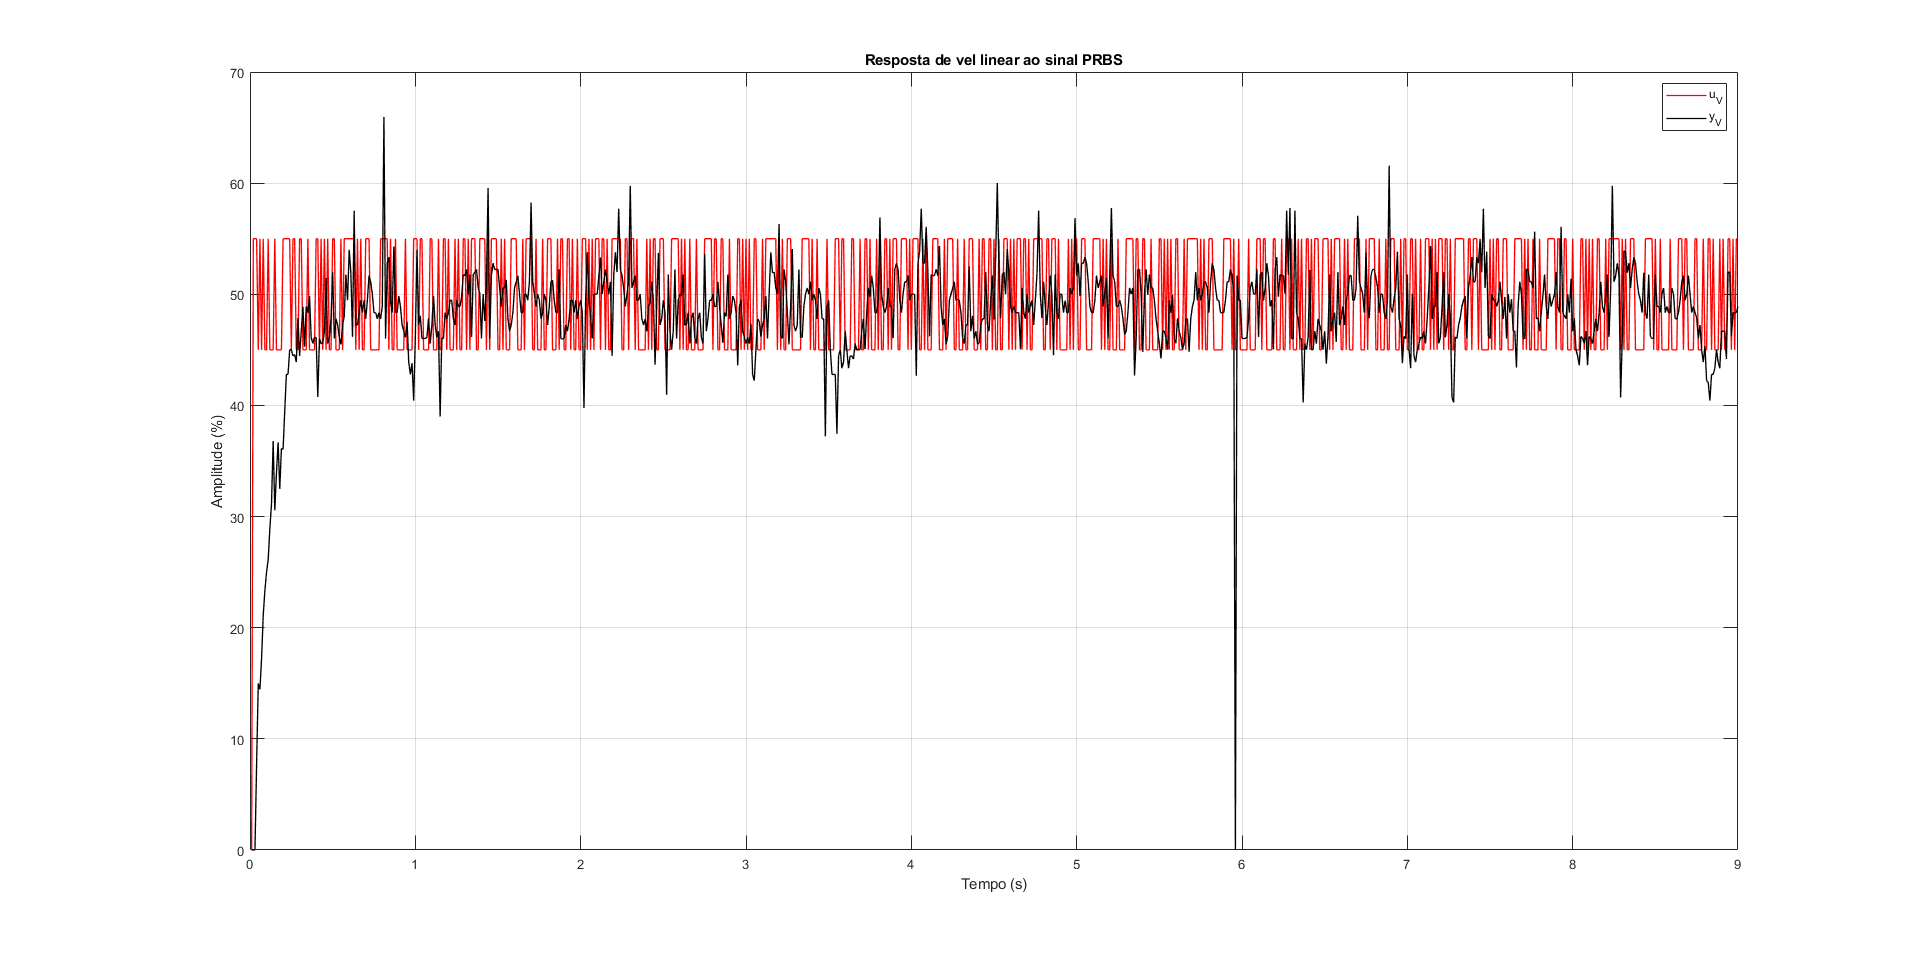
\includegraphics[width=16cm]{figuras/resultados/fig-global/resp-prbs-vel-lin.png}
                    }{
                        \Fonte{O autor}
                    }	
            \end{figure}

            \begin{figure}[ht]
                \centering
                \Caption{\label{fig:resposta-prbs-w-angular} Resposta a entrada PRBS de $\omega$}	
                    \UFCfig{}{
                        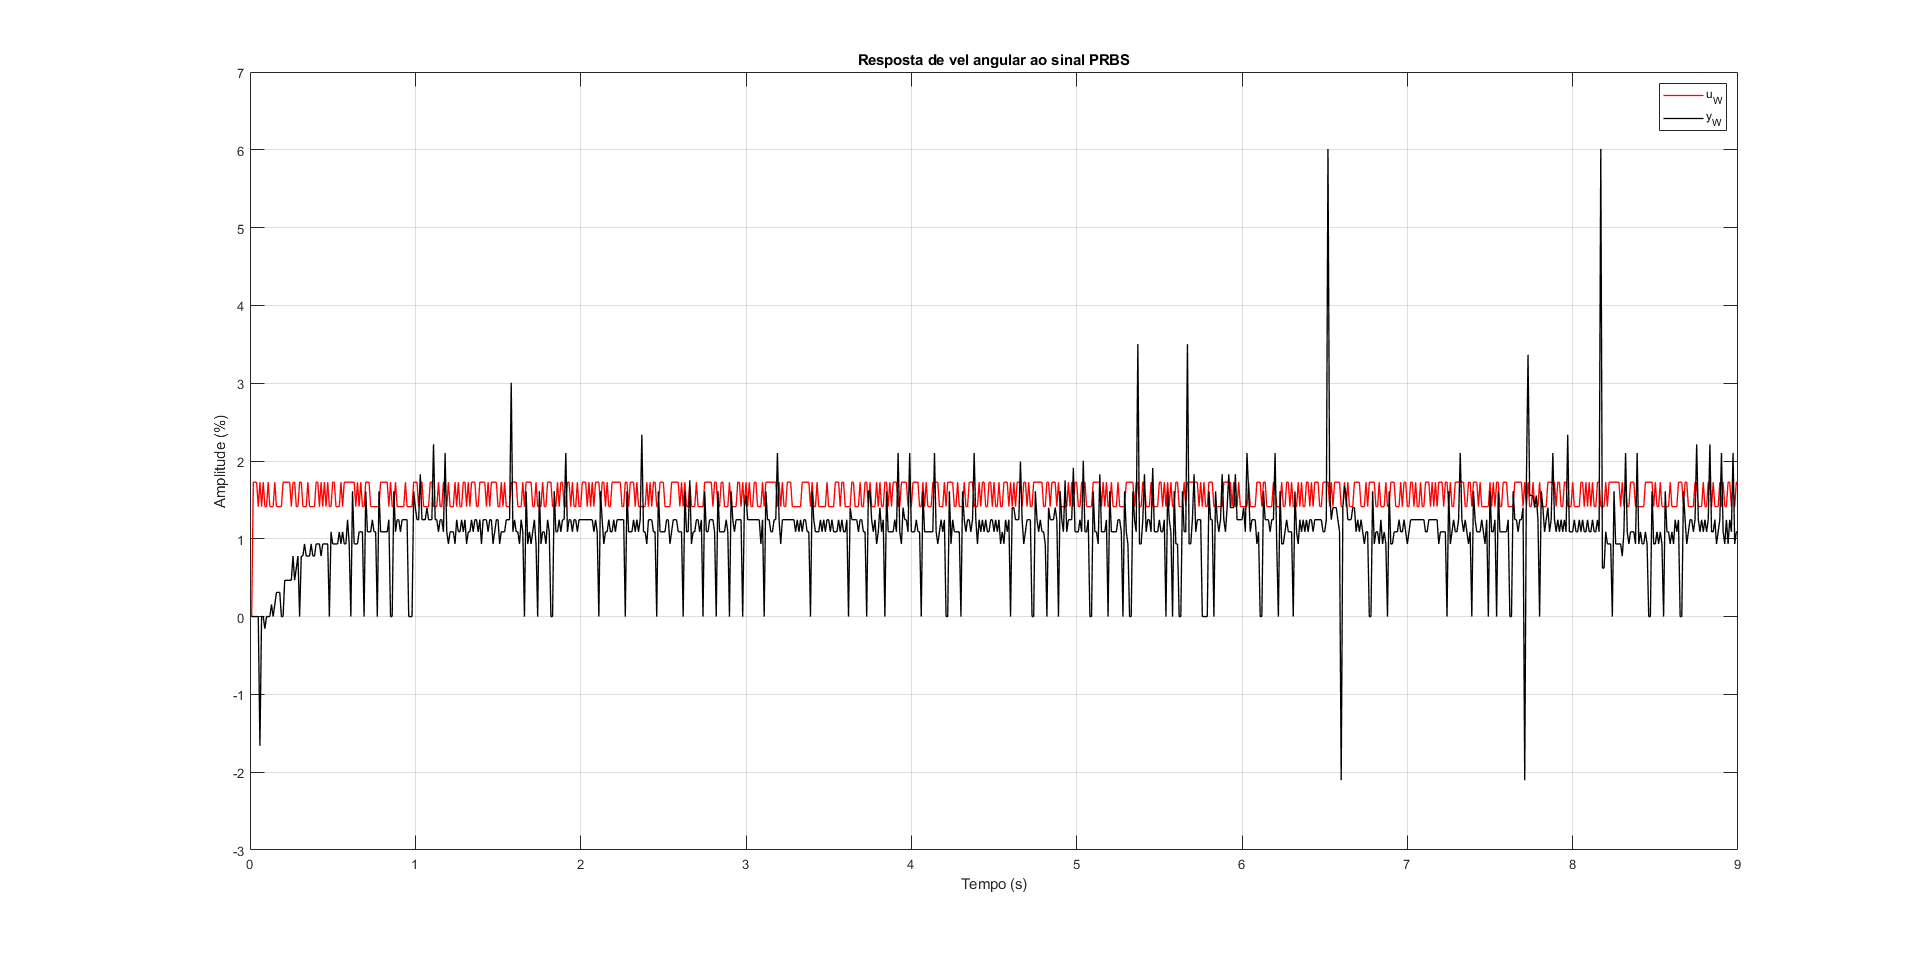
\includegraphics[width=16cm]{figuras/resultados/fig-global/resp-prbs-w-ang.png}
                    }{
                        \Fonte{O autor}
                    }	
            \end{figure}

            Semelhantemente ao realizado nos motores, é aplicado o método \gls{MQNR} para identificação das malhas. Os resultados em testes de validação obtidos são apresentados nas Figuras \ref{fig:identificacao-global-v-linear} e \ref{fig:identificacao-global-w-angular} bem como os coeficientes encontrados, os quais estão presentes na Tabela \ref{tab:coeficientes-identificacao-global}.

            \begin{figure}[ht]
                \centering
                \Caption{\label{fig:identificacao-global-v-linear} Resultado da identificação da malha $V$ pelo MQNR}	
                    \UFCfig{}{
                        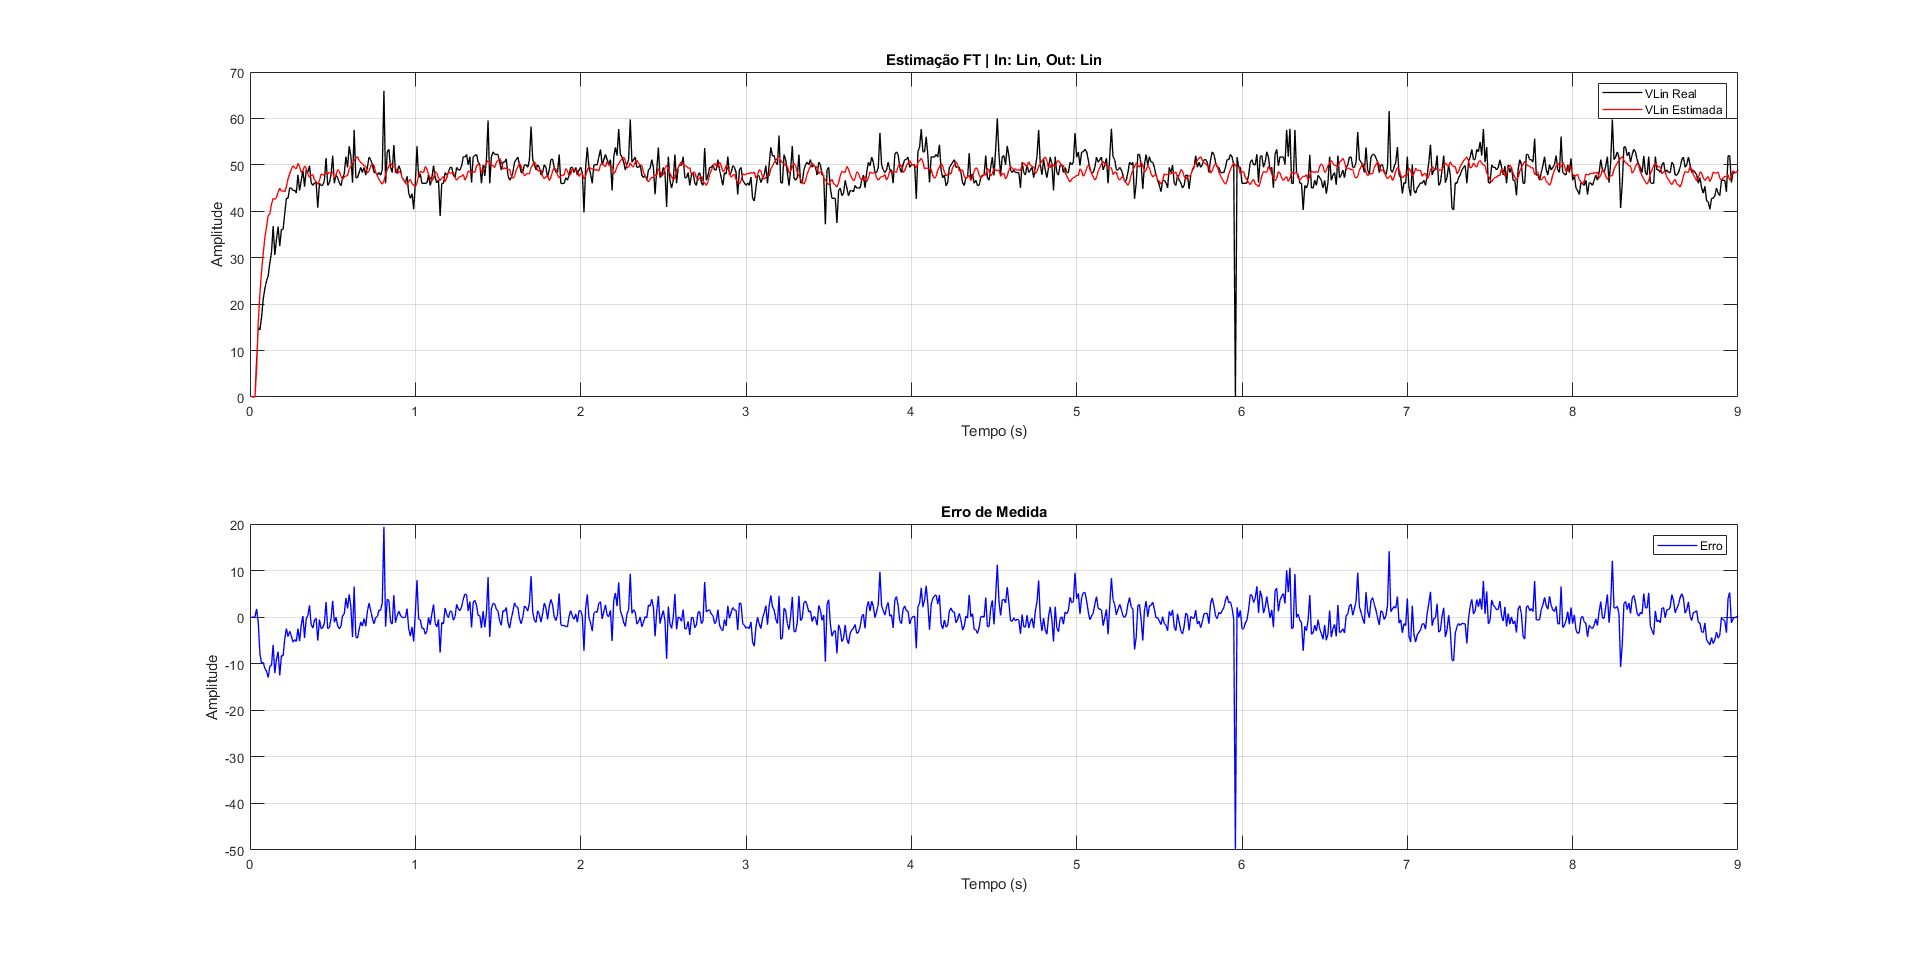
\includegraphics[width=16cm]{figuras/resultados/fig-global/identifica-vel-lin.png}
                    }{
                        \Fonte{O autor}
                    }	
            \end{figure}

            \begin{figure}[ht]
                \centering
                \Caption{\label{fig:identificacao-global-w-angular} Resultado da identificação da malha $\omega$ pelo MQNR}	
                    \UFCfig{}{
                        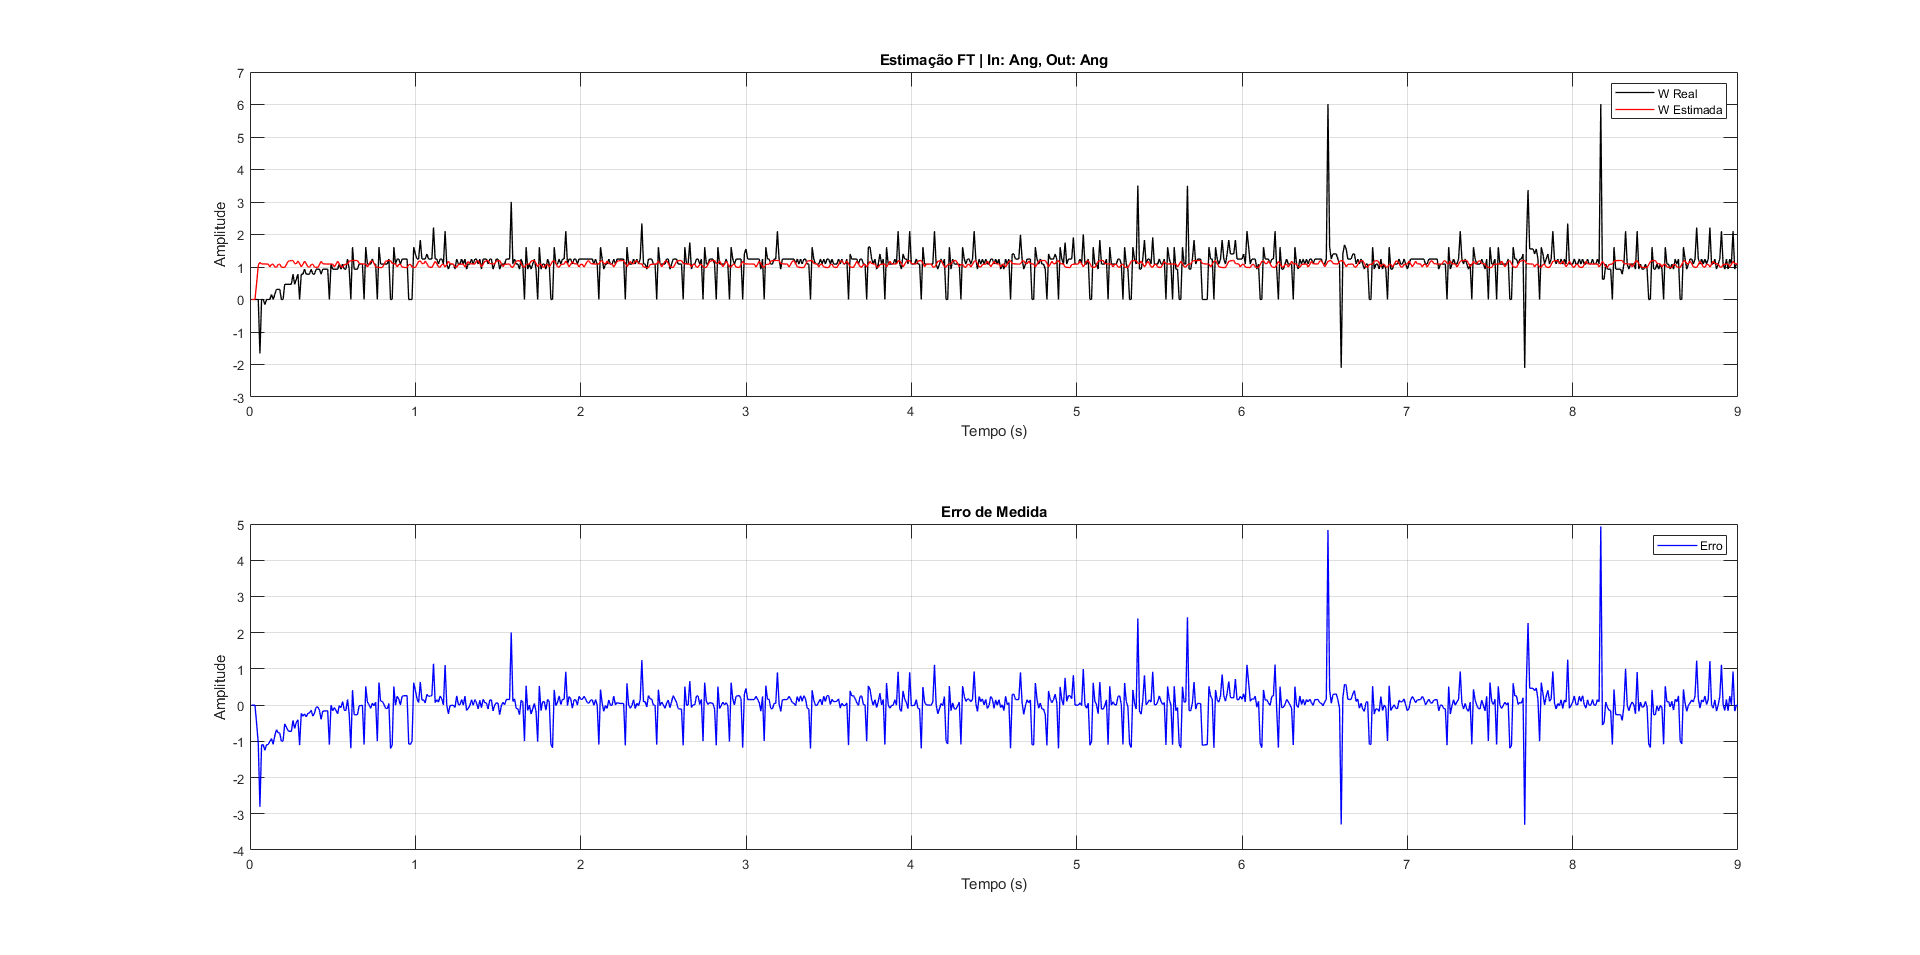
\includegraphics[width=16cm]{figuras/resultados/fig-global/identifica-w-ang.png}
                    }{
                        \Fonte{O autor}
                    }	
            \end{figure}

            \begin{table}[!htbp]	
				\centering
				\Caption{\label{tab:coeficientes-identificacao-global} Coeficientes dos modelos das malhas globais}
				\UFCtab{}{
					\begin{tabular}{ccc}
						\toprule
						Coeficiente/Malha & \( V \) & \( \omega  \) \\
						\midrule
						\( a_1 \) & \( -0.4089 \) & \( -0.1054 \) \\
						\( a_2 \)    & \( -0.3344 \) & \( -0.0578 \) \\
						\( b_1 \)   & \( 0.1094 \) & \( 0.2874 \) \\
                        \( b_2 \)   & \( 0.1397 \) & \( 0.2940 \) \\
						\bottomrule
					\end{tabular}
				}{
					\Fonte{O autor}
				}
			\end{table}

        \subsection{Controle aplicado nas variáveis globais} \label{sec:res-controle-global}

            Tendo sido modeladas as malhas de velocidade linear ($V$) e velocidade angular ($\omega$) é realizado a aplicação do método do Relé novamente, para cada uma das malhas, como apresentado nas Figuras \ref{fig:rele-vel-linear} e \ref{fig:rele-w-angular}, em seguida são determinados seus parâmetros os quais estão sintetizados na tabela \ref{tab:parametros-rele-global}.

            \begin{figure}[ht]
                \centering
                \Caption{\label{fig:rele-vel-linear} Aplicação do relé na malha $V$}	
                    \UFCfig{}{
                        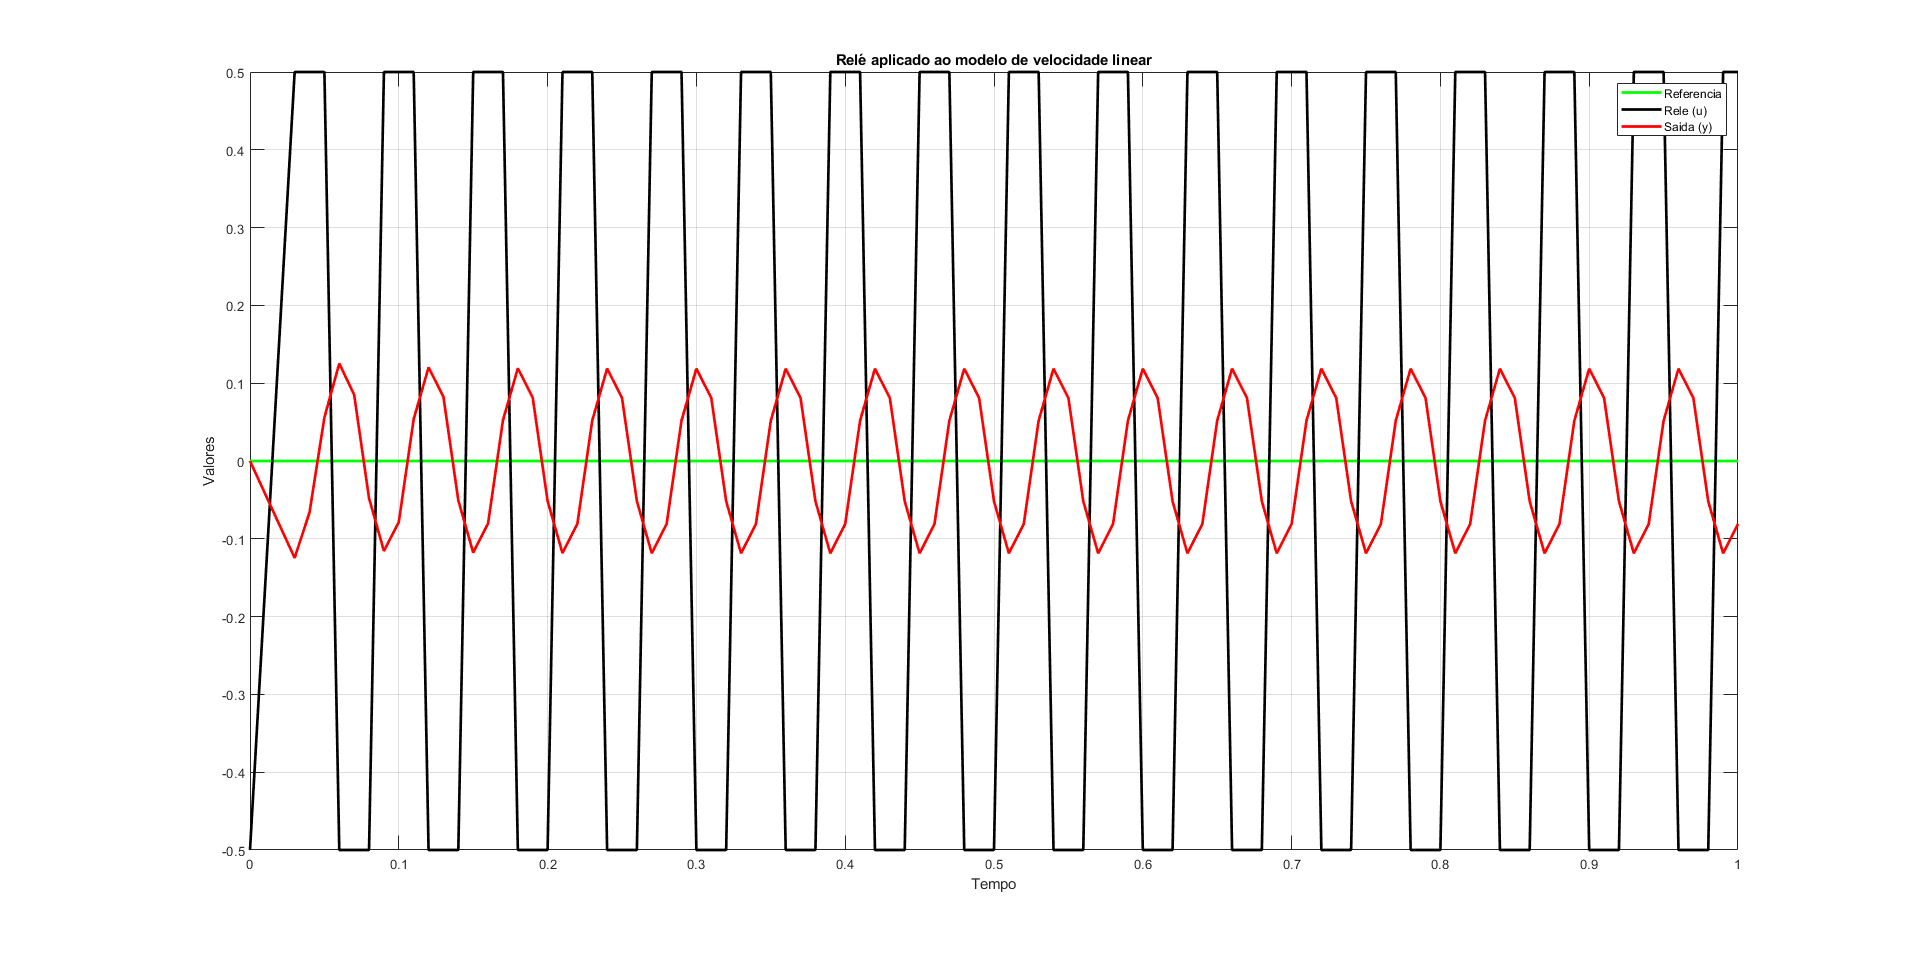
\includegraphics[width=16cm]{figuras/resultados/fig-global/rele-vel-lin.png}
                    }{
                        \Fonte{O autor}
                    }	
            \end{figure}

            \begin{figure}[ht]
                \centering
                \Caption{\label{fig:rele-w-angular} Aplicação do relé na malha $\omega$}	
                    \UFCfig{}{
                        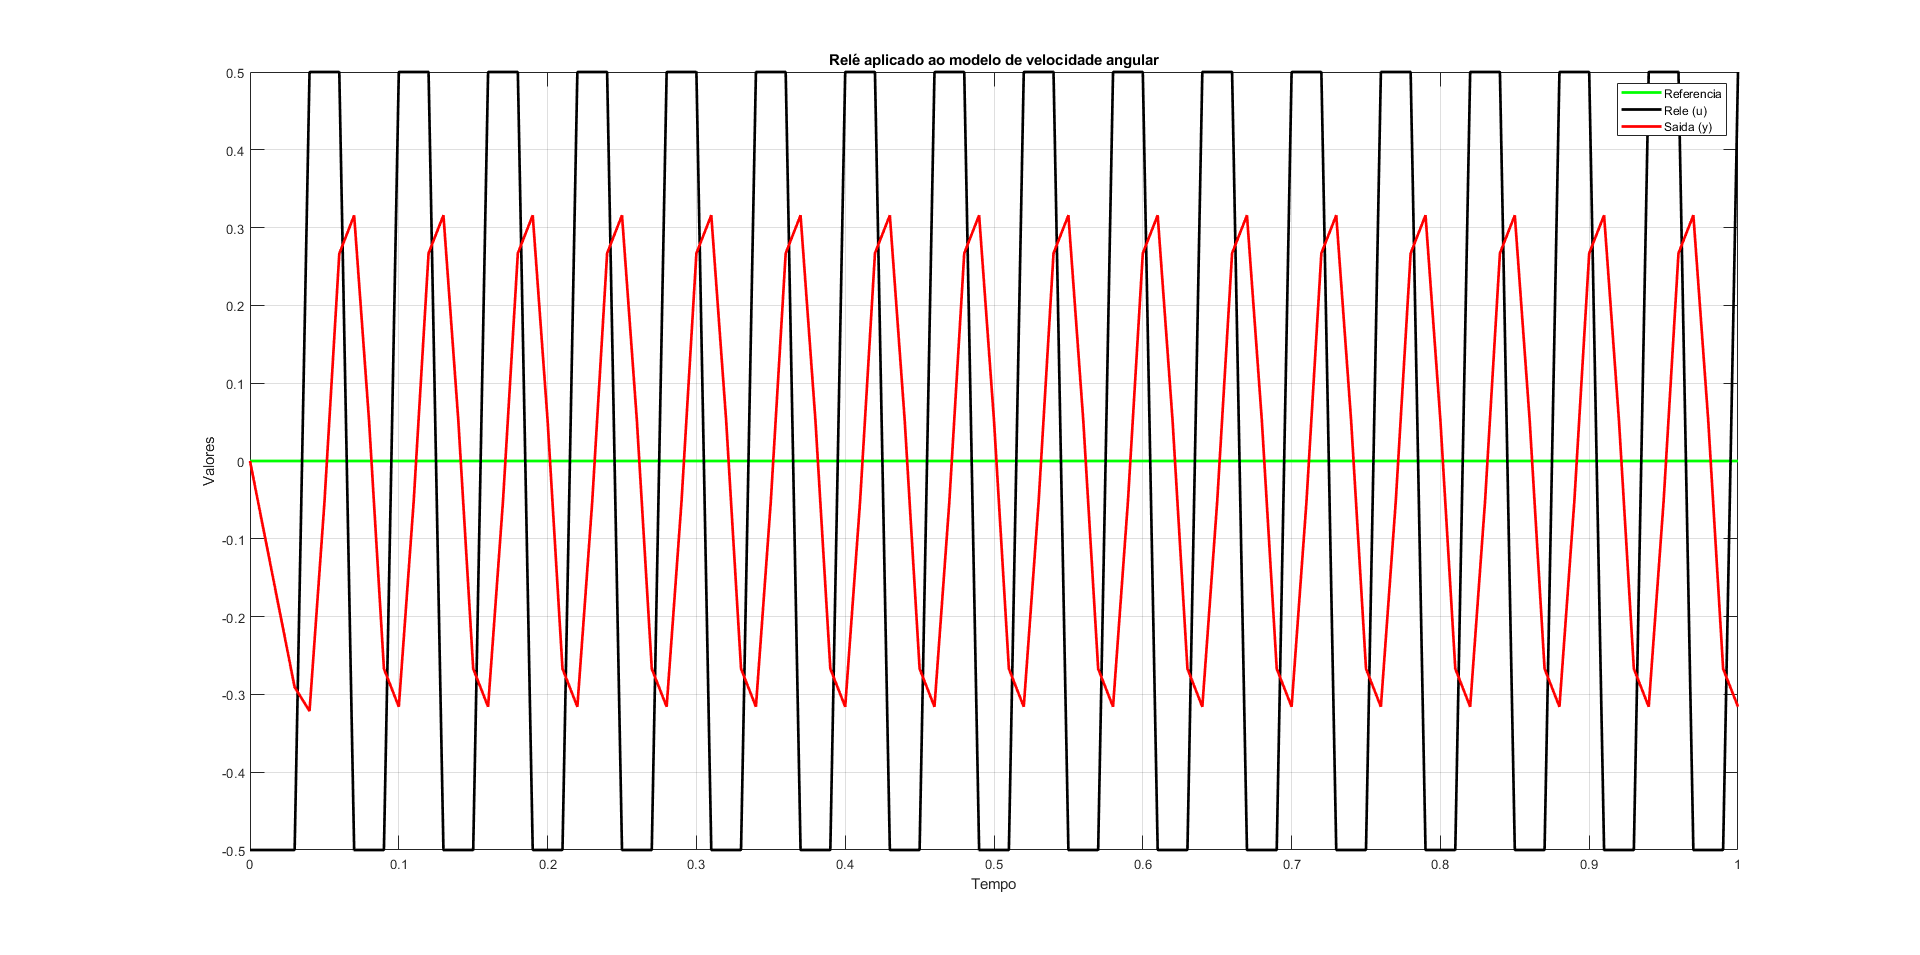
\includegraphics[width=16cm]{figuras/resultados/fig-global/rele-w-ang.png}
                    }{
                        \Fonte{O autor}
                    }	
            \end{figure}

            \begin{table}[!htbp]	
				\centering
				\Caption{\label{tab:parametros-rele-global} Parâmetros do Relé para as malhas globais}
				\UFCtab{}{
					\begin{tabular}{ccc}
						\toprule
						    Parâmetro/Malha & \( V \) & \( \omega \) \\
						\midrule
                            \( K_{u} \) & \( 5.2831 \) & \( 2.0111 \) \\
                            \( T_{u} \)    & \( 0.0600 \) & \( 0.0600 \) \\
                            \( a \)   & \( 0.1205 \) & \( 0.3165 \) \\
                            \( d \)   & \( 0.5000 \) & \( 0.5000 \) \\
                            \( \epsilon \)   & \( 0.1 \) & \( 0.29  00 \) \\
                            \( \omega_{u} \)   & \( 104.7198 \) & \( 104.7198 \) \\
						\bottomrule
					\end{tabular}
				}{
					\Fonte{O autor}
				}
			\end{table}

            No presente trabalho, por questões de limitações temporais, associadas, também, a problemas técnicos encontrados nas etapas práticas finais, não foi possível realizar a implementação prática das malhas de controle globais como foi feito com os controladores dos motores, de forma que para estas malhas estão apresentadas resultados simulados, os quais permitem ter uma compreensão de como se dará o comportamento do robô quando aplicado em condições de teste reais.

            Novamente, e de forma semelhante ao que foi apresentado para os controladores dos motores direito e esquerdo os controladores projetados são avaliados em ensaios para um e para três patamares. Os parâmetros dos controladores são apresentados na Tabela \ref{tab:parametros-controladores-global}.

            \begin{table}[!htbp]	
				\centering
				\Caption{\label{tab:parametros-controladores-global} Parâmetros dos Controladores Supervisórios}
				\UFCtab{}{
					\begin{tabular}{ccc}
						\toprule
						Parâmetro/Malha & \( V \) & \( \omega \) \\
						\midrule
						\( g_0 \) & \( 0.5839 \) & \( 1.6144 \) \\
						\( g_1 \)    & \( -0.5913 \) & \( -1.2420 \) \\
						\( g_2 \)   & \( 0.1700 \) & \( 0.3219 \) \\
						\bottomrule
					\end{tabular}
				}{
					\Fonte{O autor}
				}
			\end{table}

            Nas Figuras \ref{fig:controle-vel-linear-1-patamar} e \ref{fig:controle-w-ang-1-patamar} são apresentados os resultados dos ensaios simulados para um patamar de referência e na Tabela \ref{tab:metricas-pid-global-1-patamar} as métricas obtidas nesta situação. Para a malha de $\omega$ manteve-se a referência como sendo $\frac{\pi}{2}$ enquanto para a de $V$ a referência foi de $50\%$. Em seguida são realizados ensaios para 3 patamares e os resultados obtidos são apresentados nas Figuras \ref{fig:controle-vel-linear-3-patamar} e \ref{fig:controle-w-ang-3-patamar} bem como as métricas estão sintetizadas na Tabela \ref{tab:metricas-pid-global-3-patamar}.

            \begin{figure}[htbp]
                \centering
                \Caption{\label{fig:controle-vel-linear-1-patamar} Controle de $V$ para 1 patamar}	
                    \UFCfig{}{
                        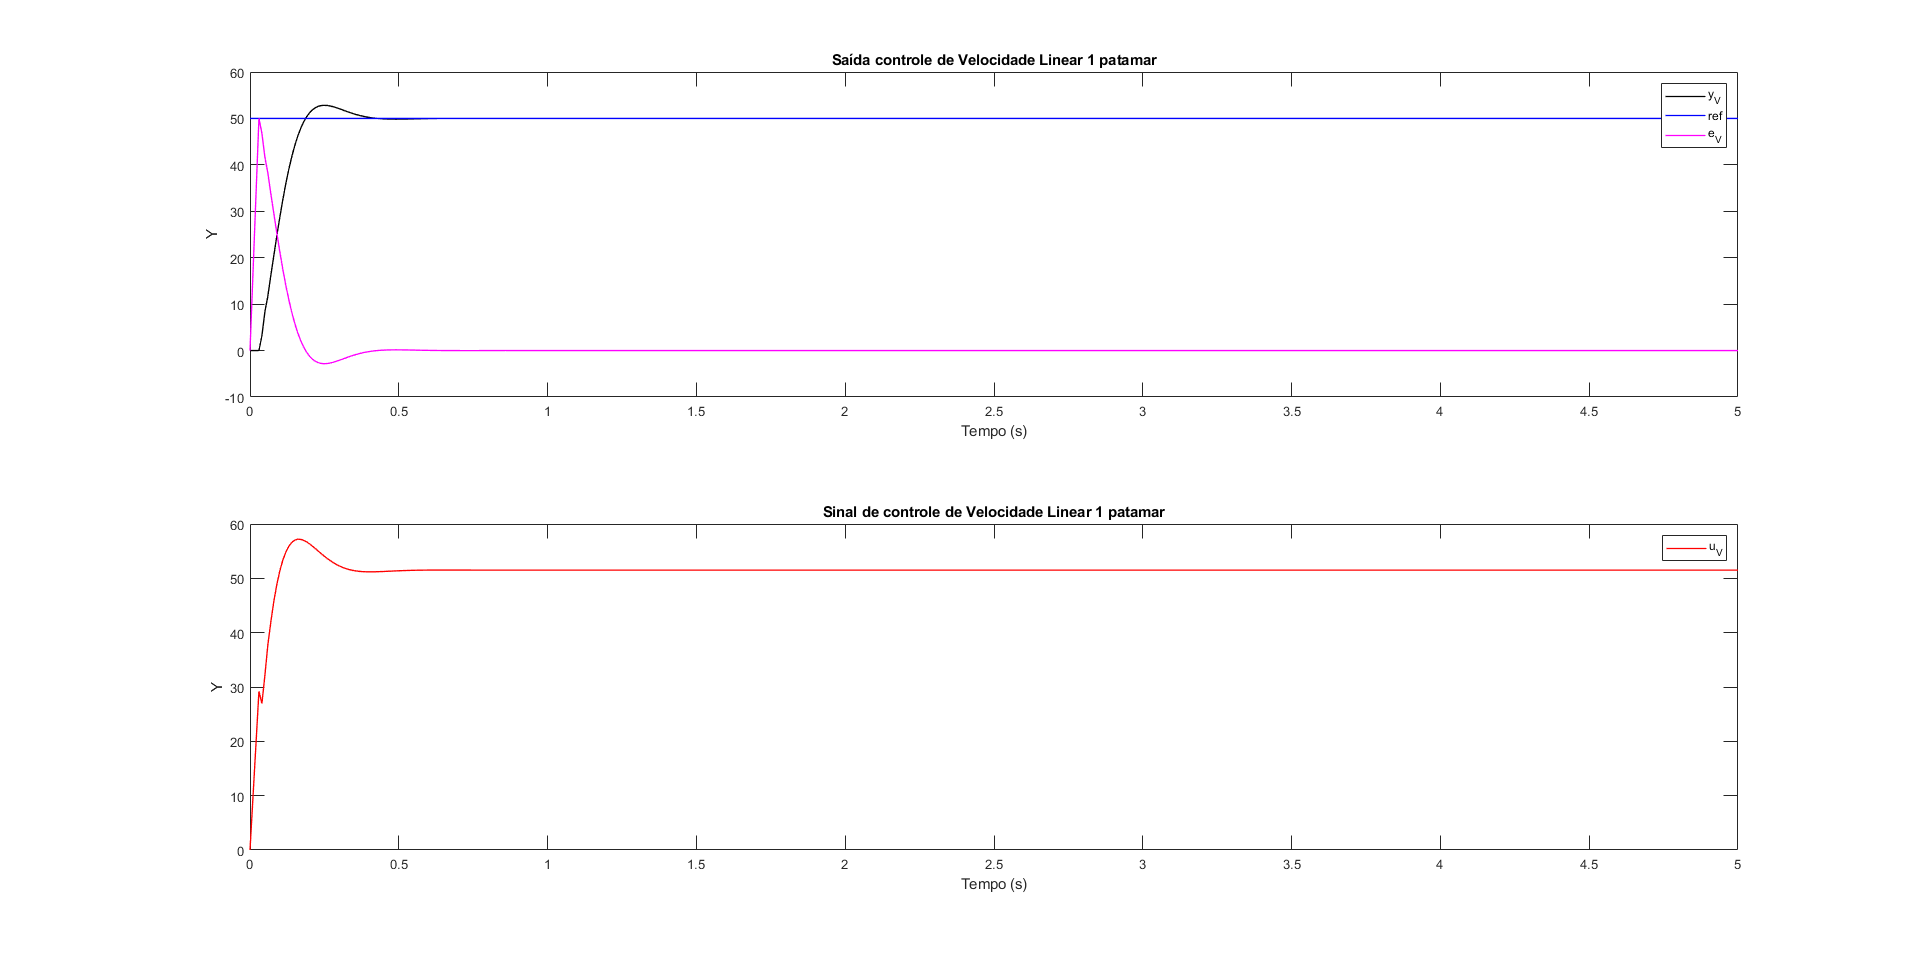
\includegraphics[width=16cm]{figuras/resultados/fig-global/contrtole-vel-lin-1-patamar.png}
                    }{
                        \Fonte{O autor}
                    }	
            \end{figure}

            \begin{figure}[htbp]
                \centering
                \Caption{\label{fig:controle-w-ang-1-patamar} Controle de $\omega$ para 1 patamar}	
                    \UFCfig{}{
                        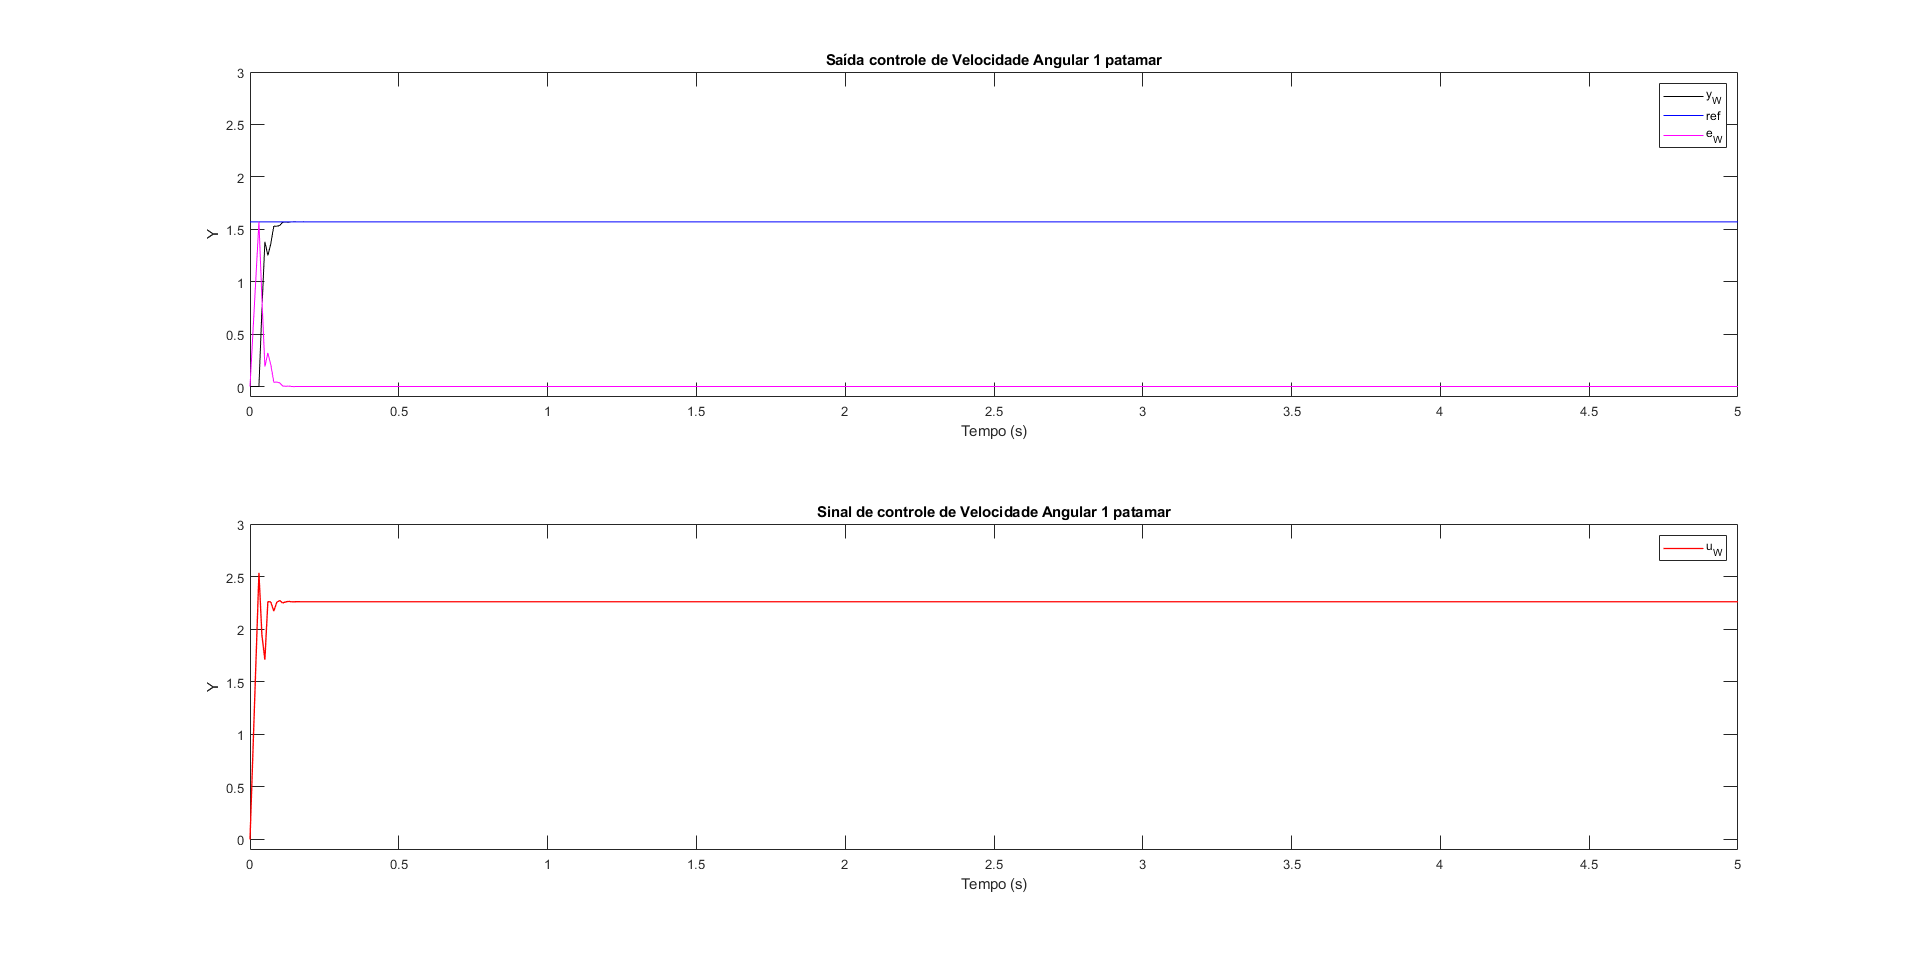
\includegraphics[width=16cm]{figuras/resultados/fig-global/contrtole-w-ang-1-patamar.png}
                    }{
                        \Fonte{O autor}
                    }	
            \end{figure}

            \begin{table}[!htbp]	
				\centering
				\Caption{\label{tab:metricas-pid-global-1-patamar} Resultados de controle para 1 patamar de $V$ e $\omega$}
				\UFCtab{}{
					\begin{tabular}{ccc}
						\toprule
						    Métrica/Malha & \( V \) & \( \omega \) \\
						\midrule
                            Sobressinal (\%) & \( 5.6565 \) & \( 0.0388 \) \\
                            IAE & \( 388.8405 \) & \( 3.2586 \) \\
                            Variância da saída & \( 33.0502 \) & \( 0.0165 \) \\
                            Variância da do controle & \( 14.7844 \) & \( 0.0214 \) \\
                            Tempo de assentamento (s) & \( 0.3200 \) & \( 0.0700 \) \\
						\bottomrule
					\end{tabular}
				}{
					\Fonte{O autor}
				}
			\end{table}

            \begin{figure}[htbp]
                \centering
                \Caption{\label{fig:controle-vel-linear-3-patamar} Controle de $V$ para 3 patamares}	
                    \UFCfig{}{
                        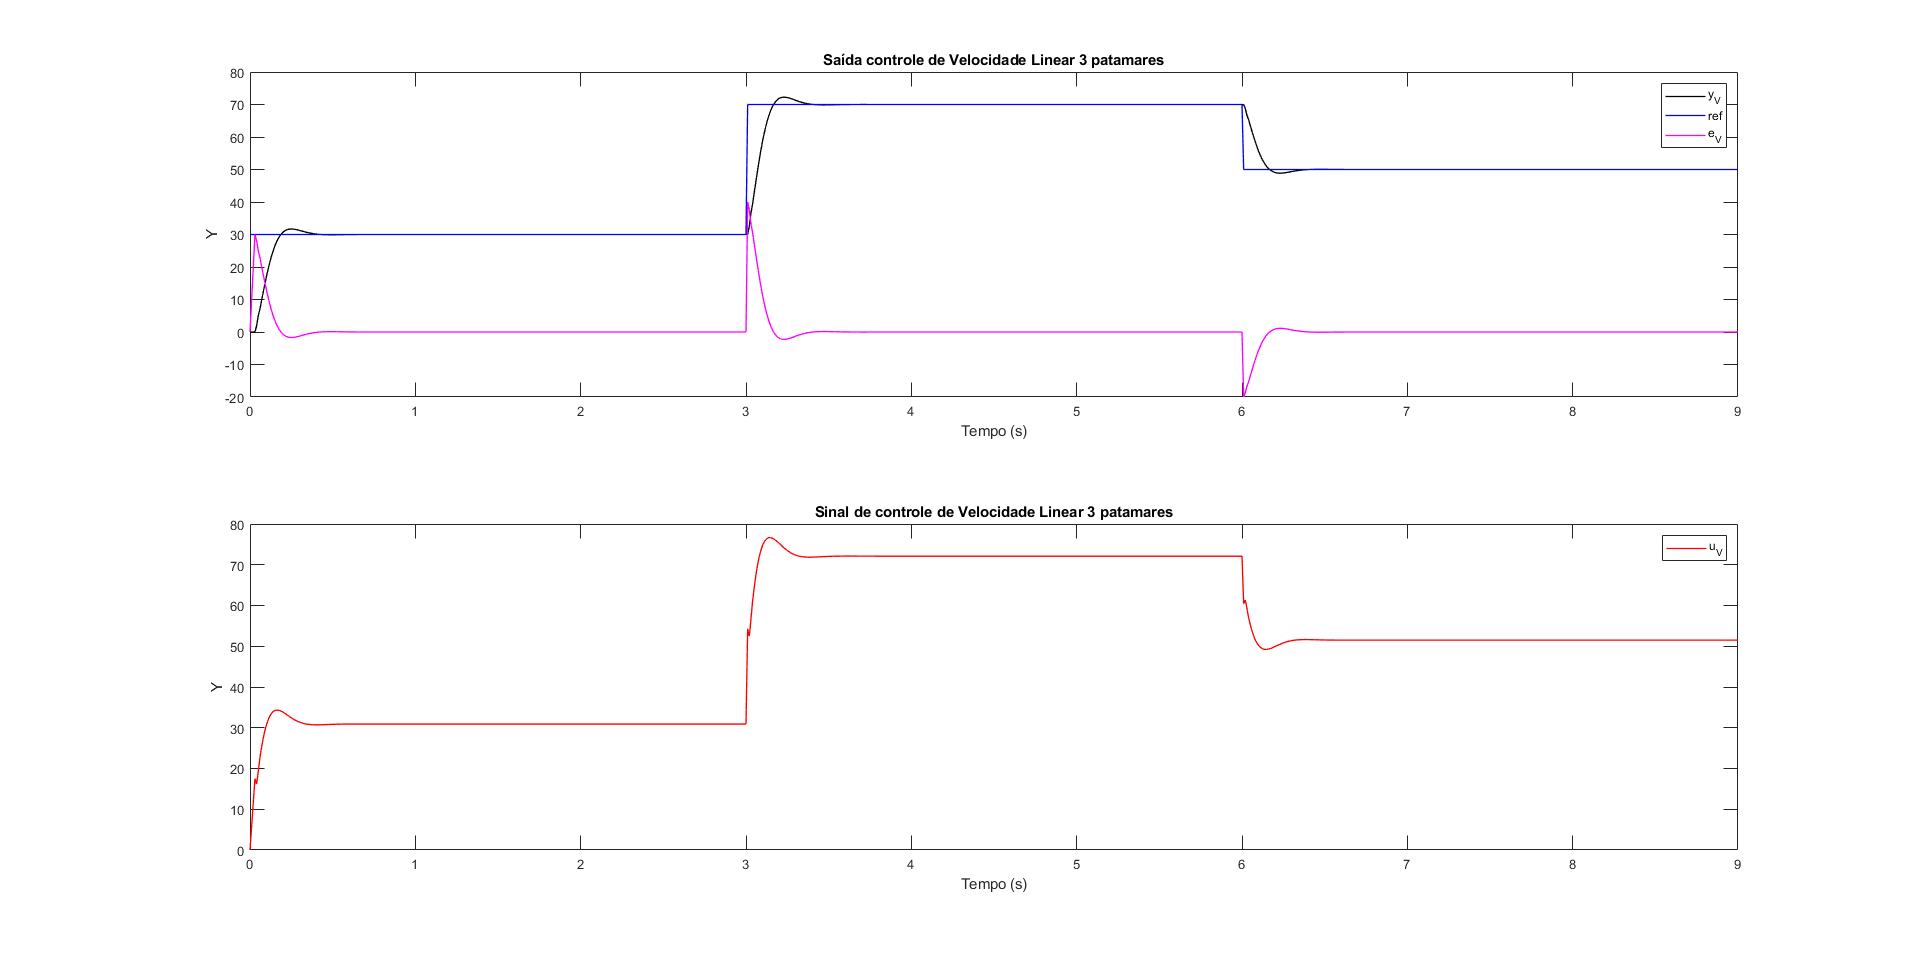
\includegraphics[width=16cm]{figuras/resultados/fig-global/contrtole-vel-lin-3-patamar.png}
                    }{
                        \Fonte{O autor}
                    }	
            \end{figure}

            \begin{figure}[htbp]
                \centering
                \Caption{\label{fig:controle-w-ang-3-patamar} Controle de $\omega$ para 3 patamares}	
                    \UFCfig{}{
                        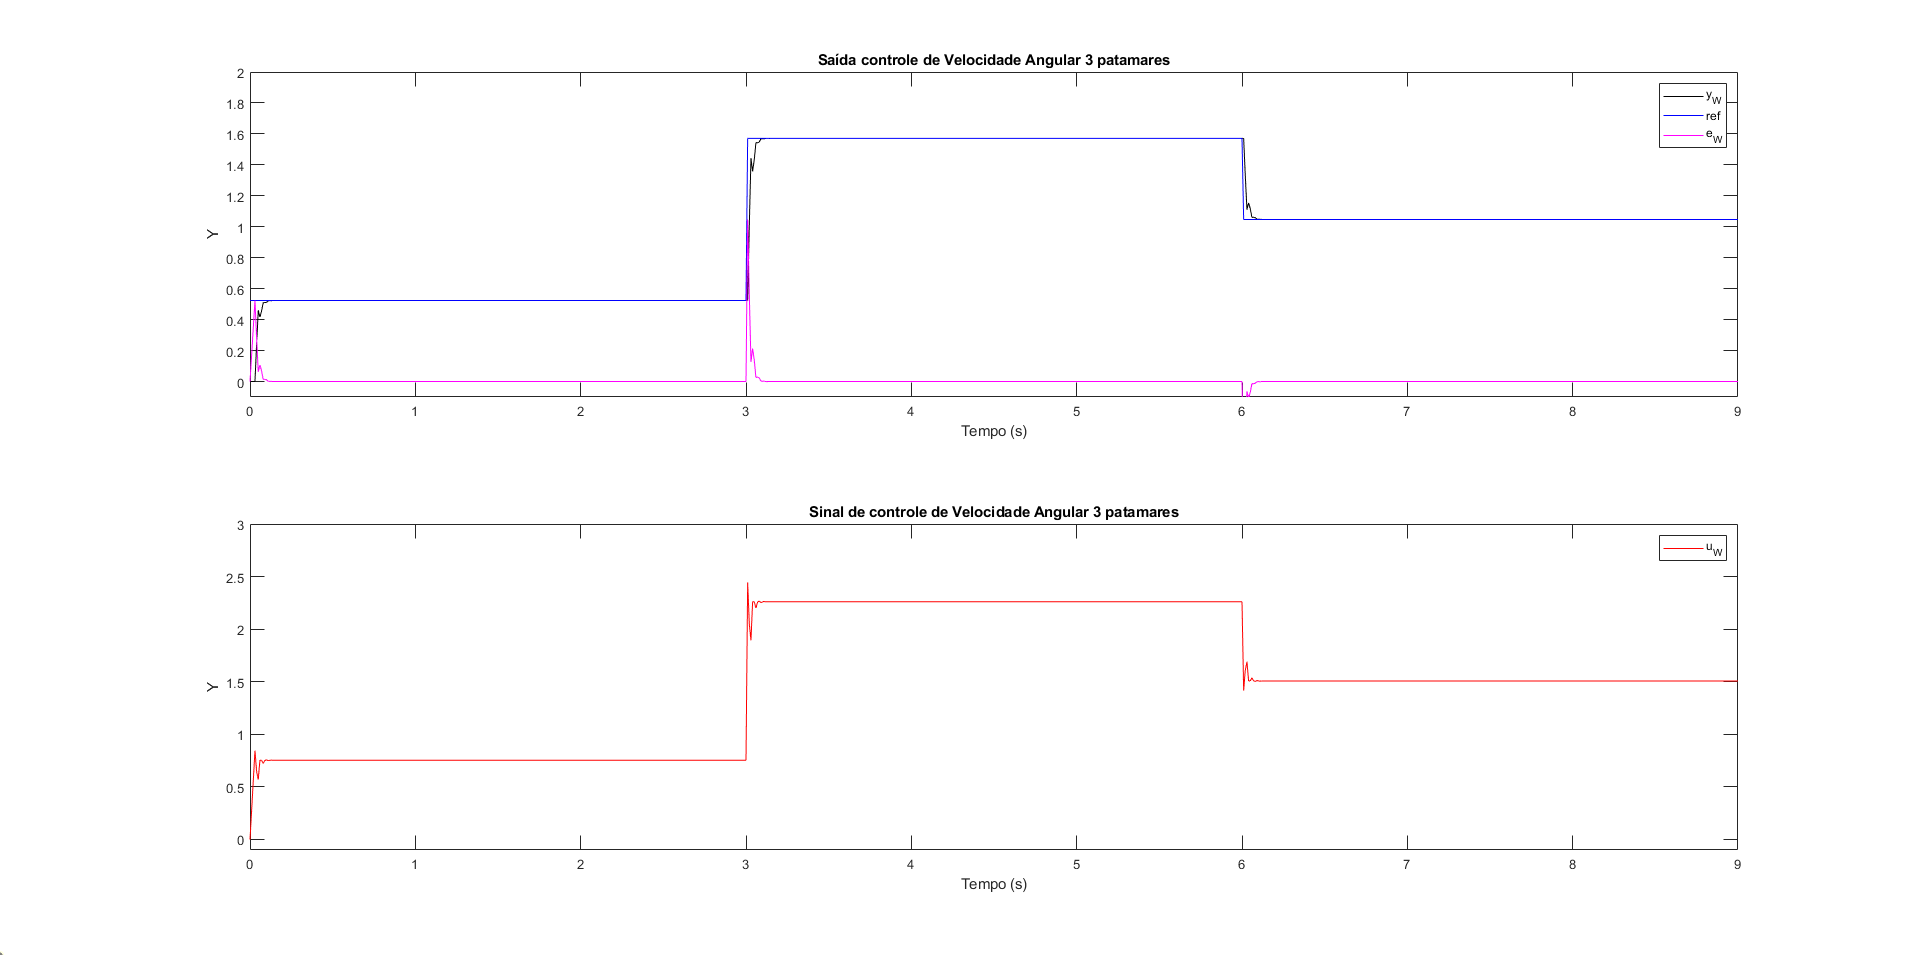
\includegraphics[width=16cm]{figuras/resultados/fig-global/contrtole-w-ang-3-patamar.png}
                    }{
                        \Fonte{O autor}
                    }	
            \end{figure}

            \begin{table}[!htbp]	
				\centering
				\Caption{\label{tab:metricas-pid-global-3-patamar} Resultados de controle supervisório para 3 patamares}
				\UFCtab{}{
					\begin{tabular}{ccc}
						\toprule
						    Métrica/Malha & \( V \) & \( \omega \) \\
						\midrule
                            Sobressinal do primeiro patamar (\%) & \( 5.6565 \) & \( 0.0388 \) \\
                            IAE & \( 699.9129 \) & \( 4.3449 \) \\
                            Variância da saída & \( 283.9178 \) & \( 0.1860 \) \\
                            Variância da do controle & \( 290.7013 \) & \( 0.3828 \) \\
                            Tempo de assentamento (s) do primeiro patamar & \( 0.3200 \) & \( 0.0500 \) \\
						\bottomrule
					\end{tabular}
				}{
					\Fonte{O autor}
				}
			\end{table}

            Tendo como ponto de análise as métricas obtidas para os controladores projetados para as malhas globais, é possível observar que o comportamento obtido encontra-se dentro do esperado haja vista que é possível interpretar as malhas globais ou supervisórias como um complemento e refino do controle realizado pelas malhas internas.